\chapter{Thiết kế và xây dựng hệ thống}

Chương này trình bày chi tiết thiết kế và triển khai thực nghiệm của hệ thống \textbf{Fiber}, 
một giải pháp tích hợp từ đầu đến cuối (end-to-end) hỗ trợ tóm tắt và kiểm chứng tin tức 
tiếng Việt. Sau phần phân tích các yêu cầu hệ thống (Mục~3.1), Mục~3.2 giới thiệu về kiến trúc 
tổng quan gồm ba dịch vụ; các Mục~3.3 đến 3.5 mô tả chi tiết các phân hệ tóm tắt và 
kiểm chứng thông tin; Mục~3.6 trình bày sâu sắc về khung đánh giá ba trục (Three-Axis Framework) 
— đóng góp chính về mặt phương pháp luận của khóa luận; Mục~3.7 mô tả thiết kế lược đồ cơ sở 
dữ liệu; và Mục~3.8 hướng dẫn chi tiết về giao diện người dùng của hệ thống.

\section{Phân tích yêu cầu hệ thống}

\subsection{Yêu cầu chức năng}

\begin{enumerate}
  \item \textbf{Tóm tắt văn bản.} Nhận đầu vào là một đường dẫn (URL) tin tức tiếng Việt, 
        trả về một bản tóm tắt tóm lược (abstractive summary) $S$ sao cho $|S| \leq 0.5 \cdot |D|$ (độ dài bản tóm tắt không quá một nửa độ dài văn bản gốc).
  \item \textbf{Truyền dữ liệu dạng luồng (Streaming).} Truyền bản tóm tắt theo từng thực thể từ (token-by-token) 
        qua kênh Sự kiện gửi từ Máy chủ (Server-Sent-Events - SSE) để đạt thời gian phản hồi dưới một giây đối với thực thể từ đầu tiên (time-to-first-token), tối ưu hóa trải nghiệm người dùng.
  \item \textbf{Kiểm chứng thông tin.} Theo yêu cầu của người dùng, phân tách bản tóm tắt thành các 
        tuyên bố nguyên tử (atomic claims), truy xuất các minh chứng trên web cho từng tuyên bố, và hiển thị điểm độ tin cậy cùng danh sách nguồn tham chiếu tương ứng.
  \item \textbf{Chuyển đổi đa mô hình.} Cho phép người dùng lựa chọn một trong mười bốn mô hình ngôn ngữ lớn (LLM) 
        được hỗ trợ tại thời điểm chạy; đồng thời lưu giữ lựa chọn cấu hình này qua các phiên làm việc.
  \item \textbf{Hệ đo lường đánh giá (Trục~A).} Sau mỗi lượt tóm tắt, tự động tính toán các chỉ số 
        ROUGE-1/2/L, BLEU, BERTScore, tỷ lệ nén, và ghi nhận kết quả vào bảng \url{evaluation_metrics}.
  \item \textbf{Dung hợp đa tác nhân (MoA fusion).} Cung cấp chế độ định tuyến \textit{dung hợp} (fusion), 
        chạy song song ba tác nhân đề xuất (proposers) và kết hợp kết quả thông qua một tác nhân tổng hợp (aggregator) GPT-4o.
  \item \textbf{Quản trị đánh giá người dùng (Human-eval admin).} Cho phép nhà nghiên cứu xây dựng các 
        tác vụ xếp hạng ẩn danh $K$ chiều (giấu danh tính mô hình) và theo dõi các số liệu thống kê tổng hợp thuộc Trục~C.
\end{enumerate}

\subsection{Yêu cầu phi chức năng}

\begin{itemize}
  \item \textbf{Độ trễ (Latency).} Thời gian phản hồi thực thể từ đầu tiên dưới 3 giây đối với 
        tác vụ tóm tắt dạng luồng trên kết nối mạng băng thông rộng; hoàn thành toàn bộ bản tóm tắt 
        dưới 10 giây đối với bài báo có độ dài $\leq 1000$ từ.
  \item \textbf{Khả năng mở rộng (Scalability).} Giao diện lập trình ứng dụng (API) phía backend không lưu trạng thái (stateless) 
        và có khả năng mở rộng ngang thông qua Vercel; phân hệ BERTScore được triển khai dưới dạng một microservice độc lập trên Hugging Face Spaces.
  \item \textbf{Bảo mật khóa API.} Tất cả các khóa nhà cung cấp dịch vụ LLM đều được lưu trữ an toàn phía máy chủ; 
        tiện ích mở rộng (browser extension) không bao giờ tiếp cận các khóa API này.
  \item \textbf{Tương thích đa trình duyệt.} Sử dụng chuẩn Manifest V3, được kiểm thử và xác thực hoạt động ổn định trên Google Chrome và Microsoft Edge.
  \item \textbf{Theo dõi chi phí.} Mỗi lượt gọi API tới LLM đều ghi lại chi phí thực tế theo đơn vị USD 
        vào bảng số liệu đo lường để phục vụ mục đích kiểm soát ngân sách.
\end{itemize}

\section{Kiến trúc tổng quan hệ thống}

Kiến trúc của hệ thống Fiber bao gồm ba dịch vụ chính hoạt động phối hợp chặt chẽ (Hình~\ref{fig:architecture}). 
Tiện ích mở rộng trên trình duyệt (browser extension) giao tiếp với backend Next.js thông qua các giao thức REST và SSE; 
backend chịu trách nhiệm tương tác với các nhà cung cấp dịch vụ LLM thương mại và microservice BERTScore; 
toàn bộ trạng thái dữ liệu lưu trữ bền vững được quản lý bởi cơ sở dữ liệu PostgreSQL trên nền tảng Supabase.

\begin{figure}[H]
  \centering
  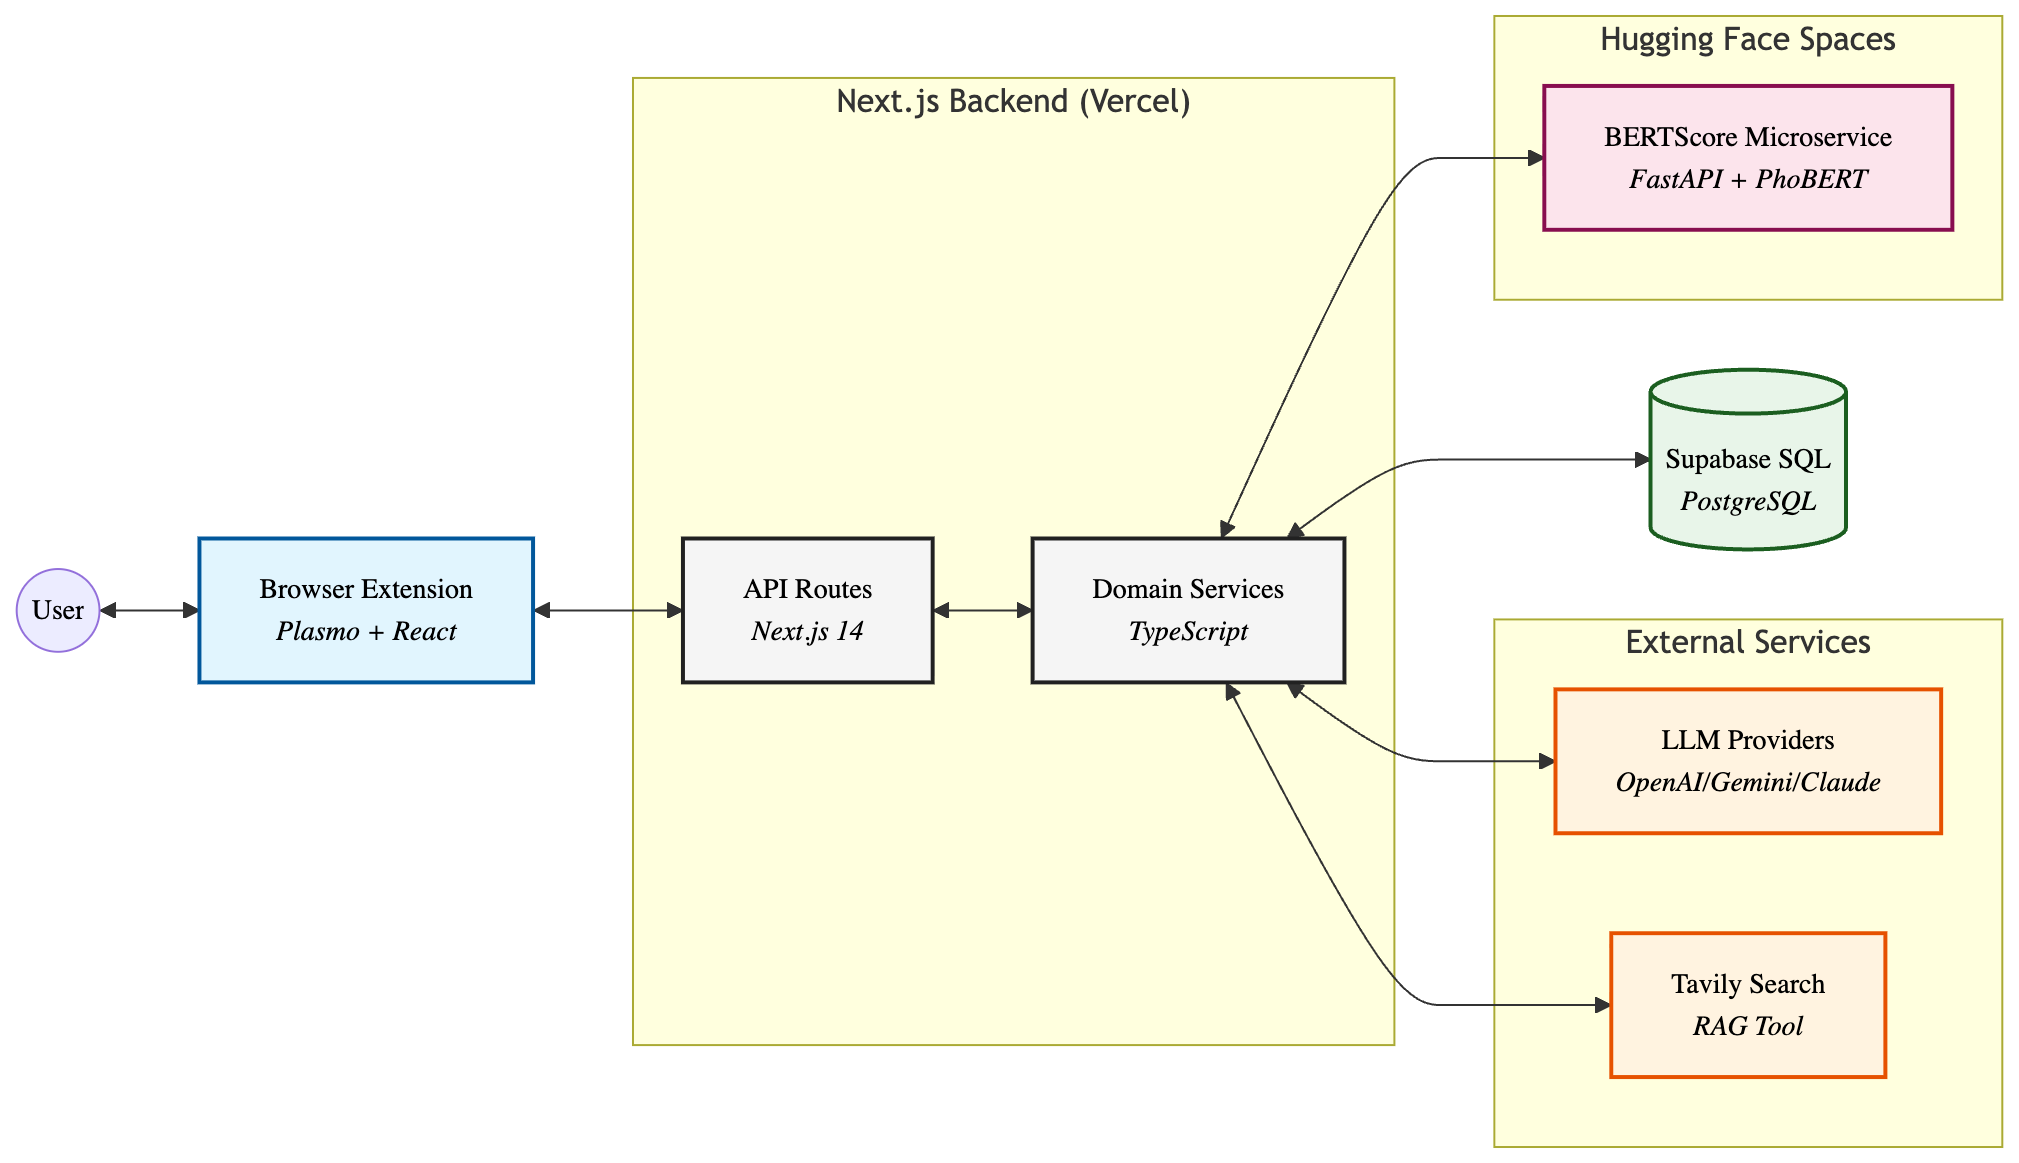
\includegraphics[width=0.85\linewidth]{figures/architecture.png}
  \caption{Kiến trúc hệ thống ba dịch vụ của Fiber.}
  \label{fig:architecture}
\end{figure}

\subsection{Tiện ích mở rộng trình duyệt (Plasmo)}

Tiện ích mở rộng được phát triển bằng ngôn ngữ TypeScript sử dụng khung phát triển Plasmo và React. Hệ thống vận hành dựa trên ba ngữ cảnh thực thi (runtime contexts) chuyên biệt:

\begin{itemize}
  \item \textit{Content script.} Chạy trực tiếp trong ngữ cảnh trang web người dùng đang truy cập; có nhiệm vụ trích xuất nội dung bài viết thông qua thư viện Mozilla Readability, nhúng một thanh bên (sidebar) được cô lập bằng cơ chế Shadow DOM nhằm tránh xung đột CSS của trang gốc, và chuyển tiếp các tương tác của người dùng tới service worker nền.
  \item \textit{Popup.} Giao diện người dùng nhỏ gọn hỗ trợ chuyển đổi mô hình nhanh chóng, cấu hình các tùy chọn và xem lịch sử sử dụng.
  \item \textit{Background service worker.} Điều phối các yêu cầu của người dùng tới hệ thống backend, quản lý luồng dữ liệu SSE, và lưu giữ trạng thái phiên làm việc thông qua API \url{chrome.storage}.
\end{itemize}

\subsection{Backend API (Next.js 14)}

Hệ thống backend được xây dựng trên mô hình Next.js App Router. Mỗi tuyến đường (route) API dạng \url{/api/...} 
đều thực hiện xác thực nghiêm ngặt dữ liệu đầu vào bằng lược đồ Zod (\texttt{backend/domain/}\allowbreak\texttt{schemas.ts}), 
sau đó ủy thác xử lý cho dịch vụ nghiệp vụ tương ứng trong thư mục \texttt{backend/}\allowbreak\texttt{services/}, 
và trả về phản hồi JSON hoặc SSE được định kiểu tĩnh. Lược đồ Zod đóng vai trò là hợp đồng dữ liệu nguồn duy nhất (single source of truth) giữa máy khách và máy chủ, loại bỏ hoàn toàn các lỗi tích hợp dữ liệu tiềm ẩn.

Các API chính bao gồm:

\begin{itemize}
  \item \url{/api/summarize} --- Thực hiện tóm tắt văn bản bằng LLM, hỗ trợ chế độ dạng luồng hoặc chế độ hàng loạt (batch).
  \item \url{/api/fact-check} --- Thực hiện kiểm chứng tính xác thực thông tin được tăng cường tìm kiếm.
  \item \url{/api/metrics} --- Các thao tác CRUD (tạo, đọc, cập nhật, xóa) trên các bản ghi đo lường chất lượng.
  \item \url{/api/human-eval/*} --- Các điểm cuối (endpoints) tiếp nhận tác vụ và phản hồi của người đánh giá thuộc Trục~C.
  \item \url{/api/settings/*} --- Cấu hình các thiết lập định tuyến, mô hình đánh giá và lựa chọn mô hình.
  \item \url{/api/logs/stream} --- Kênh SSE truyền thông tin gỡ lỗi thời gian thực phục vụ quá trình phát triển.
\end{itemize}


\subsection{Microservice BERTScore (FastAPI)}

Chỉ số BERTScore được tính toán bằng Python thông qua thư viện \url{bert_score} chính thức, 
sử dụng mô hình ngôn ngữ tiếng Việt PhoBERT làm nền tảng (\url{vinai/phobert-base}). Microservice này cung cấp một 
điểm cuối \texttt{POST} \url{/calculate-score} duy nhất và được đóng gói Docker triển khai trên Hugging Face Spaces. 
Văn bản đầu vào được cắt ngắn còn tối đa 256 từ tố (tokens) trước khi tính điểm; quá trình cắt ngắn này được thực hiện ở phía microservice 
để backend Next.js chỉ cần gửi trực tiếp hai chuỗi văn bản cần so sánh mà không cần xử lý từ tố phức tạp ở Node.js.

\section{Phân hệ tóm tắt văn bản}

Phân hệ tóm tắt văn bản được thiết kế độc lập với mô hình (model-agnostic) và hoạt động bền vững trước nhiều độ dài đầu vào khác nhau. 
Quy trình tóm tắt tuân theo một luồng công việc hệ thống từ khâu trích xuất nội dung cho đến bước đánh giá không đồng bộ.

\subsection{Quy trình tóm tắt văn bản}

Quy trình tóm tắt được điều phối nhịp nhàng thông qua cơ chế phân tách trách nhiệm rõ ràng (clear separation of concerns) 
giữa tiện ích trình duyệt phía máy khách và API Next.js phía máy chủ. 
Như minh họa trong Hình~\ref{fig:summarization_flow}, tác vụ tóm tắt có thể được kích hoạt qua hai cơ chế: 
(1) \textbf{Thanh bên tự động (Auto Sidebar)}, tự động nhận diện trang bài báo khi tải để cung cấp bản tóm tắt toàn diện, 
và (2) Hệ thống \textbf{Khung hội thoại kiểm chứng (Fact-check Modal)}, trong đó người dùng bôi đen các phân đoạn văn bản cụ thể để kích hoạt một tooltip tóm tắt theo nhu cầu. 
Các yêu cầu này được gửi tới tuyến đường \url{/api/summarize} ở backend, nơi \texttt{Summarize Service} tương tác với LLM và xác thực kết quả đầu ra qua thư viện Zod trước khi gửi lại cho giao diện người dùng tiện ích mở rộng.

Quy trình tóm tắt từ đầu đến cuối gồm năm giai đoạn chính:

\begin{enumerate}
    \item \textbf{Trích xuất (Extraction):} Khi trang web tải xong, tập kịch bản nội dung (content script) sử dụng thư viện Mozilla Readability để phân tích cú pháp DOM, loại bỏ các phần rác như quảng cáo, menu điều hướng để cô lập phần tiêu đề và nội dung chính của bài báo.
    \item \textbf{Quyết định định tuyến (Routing Decision):} Hệ thống ước lượng số lượng từ tố (tokens) và kiểm tra chế độ định tuyến hiện hoạt của người dùng (Tự động - Auto, Bắt buộc - Forced, hoặc Dung hợp - Fusion). Điều này xác định nhà cung cấp dịch vụ LLM hoặc pipeline xử lý nào (ví dụ: MoA) sẽ được gọi.
    \item \textbf{Kỹ nghệ gợi ý (Prompt Engineering):} Một câu lệnh gợi ý (prompt) được cấu trúc động chứa văn bản gốc và các chỉ dẫn cụ thể cho tác vụ tóm tắt ý nghĩa (abstractive) bằng tiếng Việt được gửi tới mô hình đã chọn.
    \item \textbf{Thực thi và Truyền luồng (Execution and Streaming):} Mô hình tạo ra kết quả. Nếu chế độ truyền luồng được bật, các từ tố được truyền trực tiếp qua kênh SSE để hiển thị thời gian thực trên giao diện. Ngược lại, toàn bộ văn bản tóm tắt sẽ được gửi về dưới dạng một khối hoàn chỉnh.
    \item \textbf{Xác thực và Hậu xử lý (Validation and Post-processing):} Bản tóm tắt thô từ LLM được xác thực đối chiếu với một lược đồ Zod. Ngay sau khi phản hồi được gửi thành công cho người dùng, hệ thống sẽ kích hoạt một tác vụ đánh giá không đồng bộ ở chế độ nền để tính toán các chỉ số Trục~A mà không gây nghẽn giao diện người dùng.
\end{enumerate}

\begin{figure}[H]
  \centering
  
\includegraphics[width=\linewidth,height=0.8\textheight,keepaspectratio]{figures/summarization_flow.png}
  \caption{Nguyên lý hoạt động của dịch vụ tóm tắt văn bản.}
  \label{fig:summarization_flow}
\end{figure}

\subsection{Trừu tượng hóa đa nhà cung cấp LLM}

Hệ thống hỗ trợ mười bốn mô hình ngôn ngữ lớn khác nhau thuộc ba nhà cung cấp dịch vụ đám mây lớn 
(\texttt{openai}, \texttt{@google/}\allowbreak\texttt{generative-ai}, \texttt{@anthropic-ai/}\allowbreak\texttt{sdk}). 
Mô-đun \texttt{llm.}\allowbreak\texttt{service.ts} cung cấp một hàm \texttt{summarize} duy nhất chịu trách nhiệm điều phối các yêu cầu đến từng nhà cung cấp và xử lý các đặc thù kỹ thuật riêng biệt của từng API:

\begin{itemize}
  \item Các mô hình suy luận sâu (\texttt{o4-mini}) bỏ qua các tham số về nhiệt độ (temperature), top-$p$, và hình phạt tần suất (\allowbreak{frequency-penalty}).
  \item Các mô hình của Anthropic giới hạn nhiệt độ trong khoảng $[0, 1]$ và không hỗ trợ cấu hình hạt giống ngẫu nhiên (seed).
  \item Các mô hình Gemini sử dụng tùy chọn \texttt{responseMimeType:} \texttt{"application/json"} để bắt buộc trả về cấu trúc dữ liệu JSON định hình sẵn.
\end{itemize}

Chi phí cho mỗi lượt gọi API được tính toán dựa trên bảng giá niêm yết của từng nhà cung cấp dịch vụ và lưu trữ trực tiếp vào cột \url{cost_usd} của bảng \url{evaluation_metrics}. 
Tại mỗi thời điểm, chỉ một mô hình duy nhất được cấu hình hoạt động để đảm bảo tính nhất quán, điều này được ràng buộc bằng chỉ mục duy nhất một phần (partial unique index) trong bảng \url{model_configurations}.

\subsection{Định tuyến dựa trên độ phức tạp văn bản}

Đối với các bài viết tiếng Việt ngắn, việc sử dụng các mô hình nội địa tối ưu hóa cho tiếng Việt mang lại hiệu quả chi phí cao hơn và giữ ngôn ngữ tự nhiên hơn so với việc gọi các mô hình thương mại quốc tế đắt đỏ. 
Phân lớp định tuyến ước lượng độ dài đầu vào theo công thức $\lceil |D|_{\text{chars}} / 4 \rceil$ từ tố và phân bổ xử lý như sau:

\begin{itemize}
  \item $\leq 400$ từ tố $\Rightarrow$ Sử dụng mô hình tiếng Việt chuyên dụng ViT5-large.
  \item $400$--$2000$ từ tố $\Rightarrow$ Định tuyến mặc định tới GPT-4o-mini.
  \item $> 2000$ từ tố $\Rightarrow$ Sử dụng GPT-4o-mini kết hợp cơ chế phân nhỏ ngữ cảnh (chunked context).
\end{itemize}

Hệ thống cung cấp ba chế độ định tuyến chính cho người dùng:

\begin{itemize}
  \item \texttt{auto} --- Tự động định tuyến dựa trên độ phức tạp và độ dài văn bản như mô tả ở trên.
  \item \texttt{forced} --- Bắt buộc luôn luôn sử dụng mô hình do người dùng chọn thủ công.
  \item \texttt{fusion} --- Sử dụng pipeline dung hợp đa tác nhân MoA (Mục~3.4).
\end{itemize}

\subsection{Chế độ truyền luồng (Streaming) so với Chế độ hàng loạt (Batch)}

Đường truyền luồng thời gian thực được triển khai bằng giao thức Sự kiện gửi từ Máy chủ (Server-Sent Events). 
Phía backend thiết lập kết nối SSE và chuyển tiếp các đoạn văn bản (chunks) từ nhà cung cấp dưới dạng các khung `data:`; 
tiện ích mở rộng ở máy khách tiếp nhận và kết xuất (render) các từ tố lên màn hình ngay khi chúng đến nơi.

Việc tính toán các chỉ số đánh giá chất lượng (ROUGE, BLEU, và BERTScore) được kích hoạt \textit{sau khi} luồng phản hồi kết thúc hoàn toàn, 
dưới dạng một Promise chạy ngầm theo mô hình "fire-and-forget" để ghi dữ liệu bất đồng bộ vào cơ sở dữ liệu Supabase; 
thiết kế này đảm bảo độ trễ trải nghiệm thực tế của người dùng hoàn toàn độc lập với thời gian tính toán các chỉ số đánh giá vốn đòi hỏi nhiều tài nguyên.

\section{Pipeline dung hợp kết quả đa tác nhân (MoA)}

Pipeline MoA (Mixture-of-Agents) đại diện cho đóng góp kỹ thuật cốt lõi của khóa luận. 
Đây là một sự triển khai thực tế chính xác dựa trên công trình của Wang và các cộng sự \cite{Wang2024} kết hợp với một cải tiến thiết kế quan trọng: 
nhúng một đường \textit{kết nối phần dư bài viết gốc (source-article residual connection)} trực tiếp vào câu lệnh gợi ý (prompt) của tác nhân tổng hợp. 
Cải tiến này là bắt buộc vì nhiệm vụ của hệ thống là tóm tắt dựa trên ngữ cảnh thực tế (grounded summarization) thay vì chỉ tuân thủ các chỉ dẫn tự do không ràng buộc (open-ended instruction-following).

\subsection{Thiết kế hệ thống hai lớp}

Lớp~1 (các tác nhân đề xuất - proposers) gồm ba mô hình: \{\url{gpt-4o-mini}, \url{claude-haiku-4.5}, \url{gemini-2.5-flash}\}. 
Mỗi tác nhân đề xuất nhận chung một câu lệnh đầu vào: ``tóm tắt bài báo tiếng Việt này trong khoảng từ 5 đến 7 câu'' 
và độc lập tạo ra bản thảo sơ bộ $d_i$ ở chế độ song song (thực thi thông qua lệnh `Promise.all` trong JavaScript). 
Lớp~2 là tác nhân tổng hợp (aggregator) sử dụng mô hình \texttt{gpt-4o}. Tác nhân này tiếp nhận đồng thời cả văn bản bài viết gốc $D$ 
và danh sách các bản thảo sơ bộ $\{d_1, d_2, d_3\}$ để dung hợp và biên tập ra bản tóm tắt cuối cùng $S^{\star}$ (Hình~\ref{fig:moa}).

\begin{figure}[H]
  \centering
  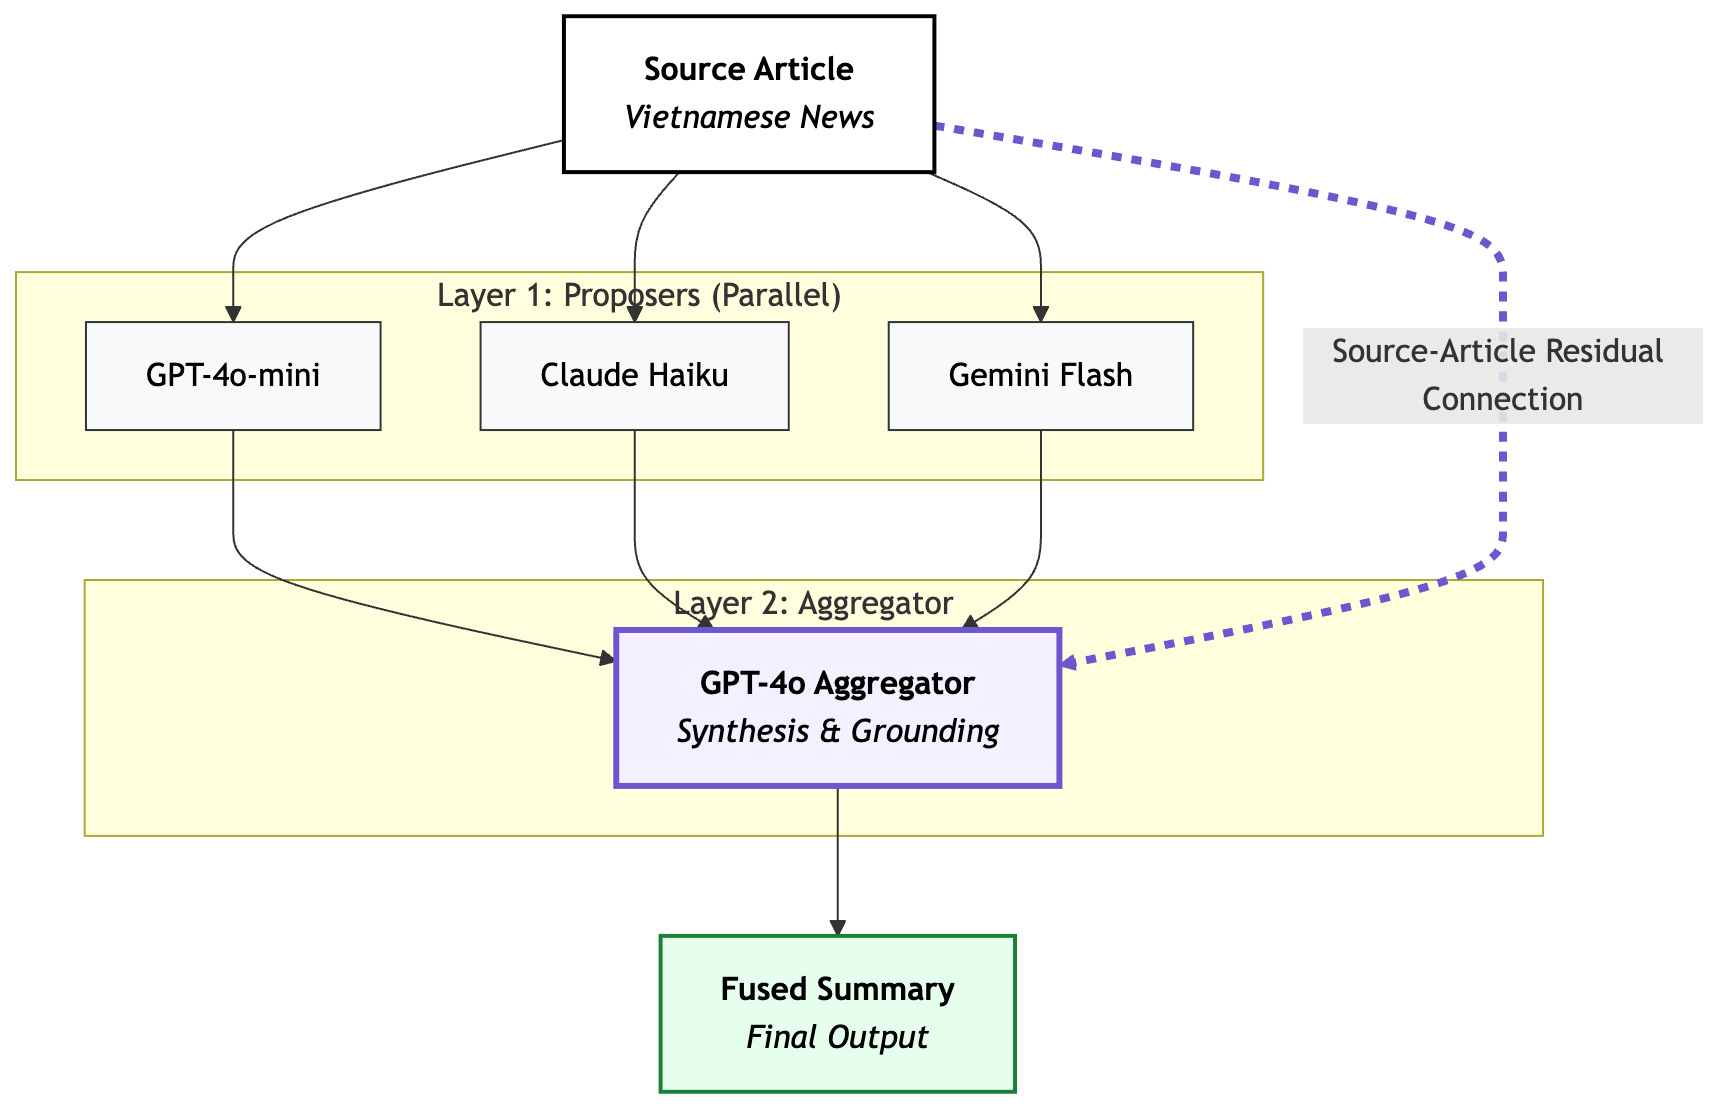
\includegraphics[width=0.85\linewidth]{figures/moa_pipeline.png}
  \caption{Kiến trúc pipeline hai lớp MoA tích hợp đường kết nối phần dư bài viết gốc.}
  \label{fig:moa}
\end{figure}

\subsection{Lớp đề xuất (Proposer Layer)}

Ba tác nhân đề xuất được tuyển chọn từ ba họ mô hình ngôn ngữ lớn thương mại đám mây khác nhau (OpenAI, Anthropic, Google) 
nhằm đảm bảo tính đa dạng trong tư duy ngôn ngữ của mô hình với chi phí vận hành cực kỳ tối ưu (cả ba đều thuộc phân khúc mô hình nhỏ gọn: \textit{mini}/\textit{haiku}/\textit{flash} của các hãng). 
Cơ chế xử lý lỗi ngoại lệ (failure handling): nếu bất kỳ một tác nhân đề xuất nào bị quá thời hạn phản hồi (timeout) hoặc trả về lỗi API, 
quá trình dung hợp vẫn tiếp tục với các bản thảo còn lại; nếu hai hoặc cả ba tác nhân đề xuất đều gặp sự cố, hệ thống sẽ trả trực tiếp bản thảo sống sót duy nhất (nếu có) và ghi lại một cảnh báo lỗi vào tệp nhật ký hệ thống.

\subsection{Lớp tổng hợp (Aggregator Layer)}

Câu lệnh gợi ý (prompt) cho tác nhân tổng hợp là cấu phần phần mềm quan trọng nhất của hệ thống triển khai thực tế; 
nó quyết định việc tác nhân tổng hợp sẽ thực hiện biên dịch sâu sắc hay chỉ đơn thuần chắp vá cơ học các bản thảo lại với nhau. 
Trong kiến trúc hiện tại, mô hình \texttt{gpt-4o} được sử dụng làm tác nhân tổng hợp. 
Câu lệnh gợi ý, sau khi được tinh chỉnh vào ngày 08-05-2026 (sự thay đổi được ghi nhận chi tiết trong commit mã nguồn \texttt{afac46e}), chỉ dẫn mô hình thực hiện:
\begin{itemize}
  \item Đánh giá các bản thảo đề xuất một cách phản biện thay vì sao chép nguyên văn;
  \item Duy trì giọng văn báo chí tiếng Việt chuẩn mực, khách quan và trung lập;
  \item Đảm bảo bản tóm tắt hoàn toàn nhất quán với bài viết gốc;
  \item \textit{Không} được sử dụng cụm từ ``cô đọng'' (tương đương với các chỉ dẫn ``condense / concise''), cụm từ mà các kết quả thực nghiệm thực tế chỉ ra rằng thường hướng mô hình tới việc tạo ra các bản tóm tắt bị cắt cụt cục bộ và thiếu tính liên kết.
\end{itemize}

\subsection{Kết nối phần dư bài viết gốc}

Phương trình~1 của nghiên cứu gốc \cite{Wang2024} chỉ thực hiện nối chuỗi câu lệnh gợi ý đầu vào với danh sách các bản thảo đề xuất. 
Đối với bài toán tóm tắt có ràng buộc thông tin thực tế, chỉ sử dụng câu lệnh gợi ý là không đủ — tác nhân tổng hợp cần bài viết gốc làm neo tham chiếu để xác thực và tổng hợp thông tin. 
Sự triển khai của chúng tôi nhúng trực tiếp toàn văn bài viết gốc vào ngữ cảnh hệ thống (system context) của tác nhân tổng hợp như một nguồn đầu vào bổ sung song song với danh sách bản thảo. 
Đây là điểm \textit{thích ứng miền (domain adaptation)} duy nhất so với công thức gốc của bài báo.

Đường kết nối phần dư này mang lại hiệu quả thực nghiệm mang tính quyết định. 
Nếu không có bài viết gốc, tác nhân tổng hợp rơi vào trạng thái chắp vá từ tố (draft-stitching) từ các bản thảo (độ dài bản tóm tắt tăng $\approx 22\%$ so với độ dài bản thảo trung bình, chỉ số ROUGE-1 so với nguồn đạt $\approx 0.34$); 
khi có sự hiện diện của bài viết gốc, tác nhân tổng hợp chuyển sang trạng thái tổng hợp biên tập (editorial synthesis) thực sự (độ dài ngắn hơn $\approx 17\%$, chỉ số ROUGE-1 giảm xuống còn $\approx 0.24$ do tính chất diễn đạt lại linh hoạt nhưng điểm đánh giá toàn diện Rubric tăng mạnh). 
Chi tiết các thực nghiệm cô lập (ablation study) này được báo cáo tại Mục~4.2.

\subsection{Thực nghiệm kỹ nghệ gợi ý đối với mô hình tổng hợp}

Ba biến thể của câu lệnh gợi ý dành cho tác nhân tổng hợp đã được thử nghiệm trên tập dữ liệu gồm 50 bài báo từ trang *tienphong.vn*:

\begin{itemize}
  \item \textbf{Baseline (Gốc)} --- Câu lệnh trước khi tinh chỉnh; không đưa bài viết gốc vào ngữ cảnh của tác nhân tổng hợp.
  \item \textbf{v1 (Strict source - Nguồn nghiêm ngặt)} --- Có đưa bài viết gốc vào ngữ cảnh, áp dụng quy tắc kiểm soát nghiêm ngặt ``không được tự ý sáng tạo thông tin''.
  \item \textbf{v2 (Soft source - Nguồn mềm dẻo)} --- Có đưa bài viết gốc vào ngữ cảnh, sử dụng các diễn đạt mềm dẻo hơn như ``sử dụng bài viết như tài liệu tham chiếu tin cậy''.
\end{itemize}

Bảng đối chiếu chi tiết các phiên bản câu lệnh gợi ý này cùng các đoạn văn bản sửa đổi cụ thể được trình bày trong Phụ lục~C.

Kết luận nổi bật nhất (được trình bày chi tiết tại Mục~4.2) chỉ ra rằng chỉ riêng sự \textit{xuất hiện} của văn bản bài viết gốc trong ngữ cảnh tổng hợp đã làm thay đổi hoàn toàn hành vi của mô hình; 
trong khi các diễn đạt câu chữ chi tiết xung quanh quy tắc đó không tạo ra sự khác biệt quá lớn. 
Phiên bản câu lệnh được tích hợp chính thức vào hệ thống là v2 cùng với việc loại bỏ từ khóa ``cô đọng'' theo cập nhật của commit \texttt{afac46e}.

\section{Phân hệ kiểm chứng sự kiện}

Phân hệ kiểm chứng sự kiện được thiết kế dưới dạng một kiến trúc RAG độc lập được điều phối trực tiếp bởi mô hình ngôn ngữ lớn. 
Quy trình kiểm chứng thông tin (Hình~\ref{fig:fact_check_flow}) được kích hoạt khi người dùng bôi đen và chọn một phân đoạn văn bản cụ thể cần xác thực. 
Giao diện \texttt{Fact-check Modal} gửi yêu cầu tới tuyến đường API \url{/api/fact-check}. 
Tại backend, \texttt{Fact-check Service} trước tiên thực hiện truy xuất minh chứng trực tuyến thông qua công cụ tìm kiếm Tavily Search 
trước khi gửi truy vấn đến LLM để đưa ra phán quyết cuối cùng. Phản hồi định kiểu tĩnh sau đó được gửi về máy khách và kết xuất trên giao diện khung hội thoại.

Quy trình xử lý tuân theo một logic tìm kiếm và xác thực hệ thống:

\begin{enumerate}
  \item Phân đoạn văn bản tóm tắt (hoặc bất kỳ đoạn văn bản tự do nào do người dùng nhập vào) được gửi tới công cụ Tavily dưới dạng một truy vấn tìm kiếm trực tuyến.
  \item Hệ thống Tavily trả về sáu kết quả tìm kiếm chất lượng cao nhất, mỗi kết quả là một bộ ba thông tin gồm \texttt{(tiêu đề bài báo, đường dẫn URL, đoạn văn bản trích dẫn)}.
  \item Các đoạn trích dẫn này, kết hợp cùng văn bản tuyên bố ban đầu của người dùng, được chuyển đến mô hình GPT-4o-mini. Mô hình phân tích và trả về một cấu trúc dữ liệu JSON gồm các trường thông tin: \url{trust_score} (điểm độ tin cậy từ $0$--$100$), \url{verified} (biến logic xác định tuyên bố đúng hay sai), và \url{sources} (danh sách các đường dẫn nguồn minh chứng).
  \item Tiện ích mở rộng tiếp nhận dữ liệu này và hiển thị trực quan trong khung hội thoại kiểm chứng ngay phía dưới bản tóm tắt.
\end{enumerate}

\begin{figure}[H]
  \centering
  
\includegraphics[width=\linewidth,height=0.8\textheight,keepaspectratio]{figures/fact_check_flow.png}
  \caption{Nguyên lý hoạt động của dịch vụ kiểm chứng thông tin được tăng cường tìm kiếm.}
  \label{fig:fact_check_flow}
\end{figure}

Việc lựa chọn mô hình GPT-4o-mini cho bước đưa ra phán quyết cuối cùng là một quyết định kỹ thuật có tính toán thực tế: 
mô hình này có chi phí vận hành rẻ hơn mười lần so với GPT-4o trong khi không ghi nhận bất kỳ sự giảm sút nào về mặt chất lượng phán quyết trên tập kiểm tra thử nghiệm gồm 50 tuyên bố thực tế.

\section{Khung đánh giá ba trục (Three-Axis Framework)}

Mục này mô tả đóng góp về mặt phương pháp luận chính của khóa luận: một khung đánh giá tích hợp đồng thời ba khía cạnh độc lập bao gồm các số liệu đo lường khả năng giữ lại nội dung (Trục~A), đánh giá chất lượng bằng mô hình ngôn ngữ lớn (Trục~B) và xếp hạng mù từ con người (Trục~C). 
Quyết định xây dựng cấu trúc đánh giá ba trục xuất phát từ các phân tích tại Mục~2.2.5: bất kỳ một trục đơn lẻ nào cũng tự bản thân nó mang những thiên kiến cấu trúc nội tại; chỉ khi kết hợp cả ba trục lại với nhau mới tạo ra một phương pháp định vị đa chiều (triangulation) đáng tin cậy để đo lường chất lượng hệ thống.

\begin{figure}[H]
  \centering
  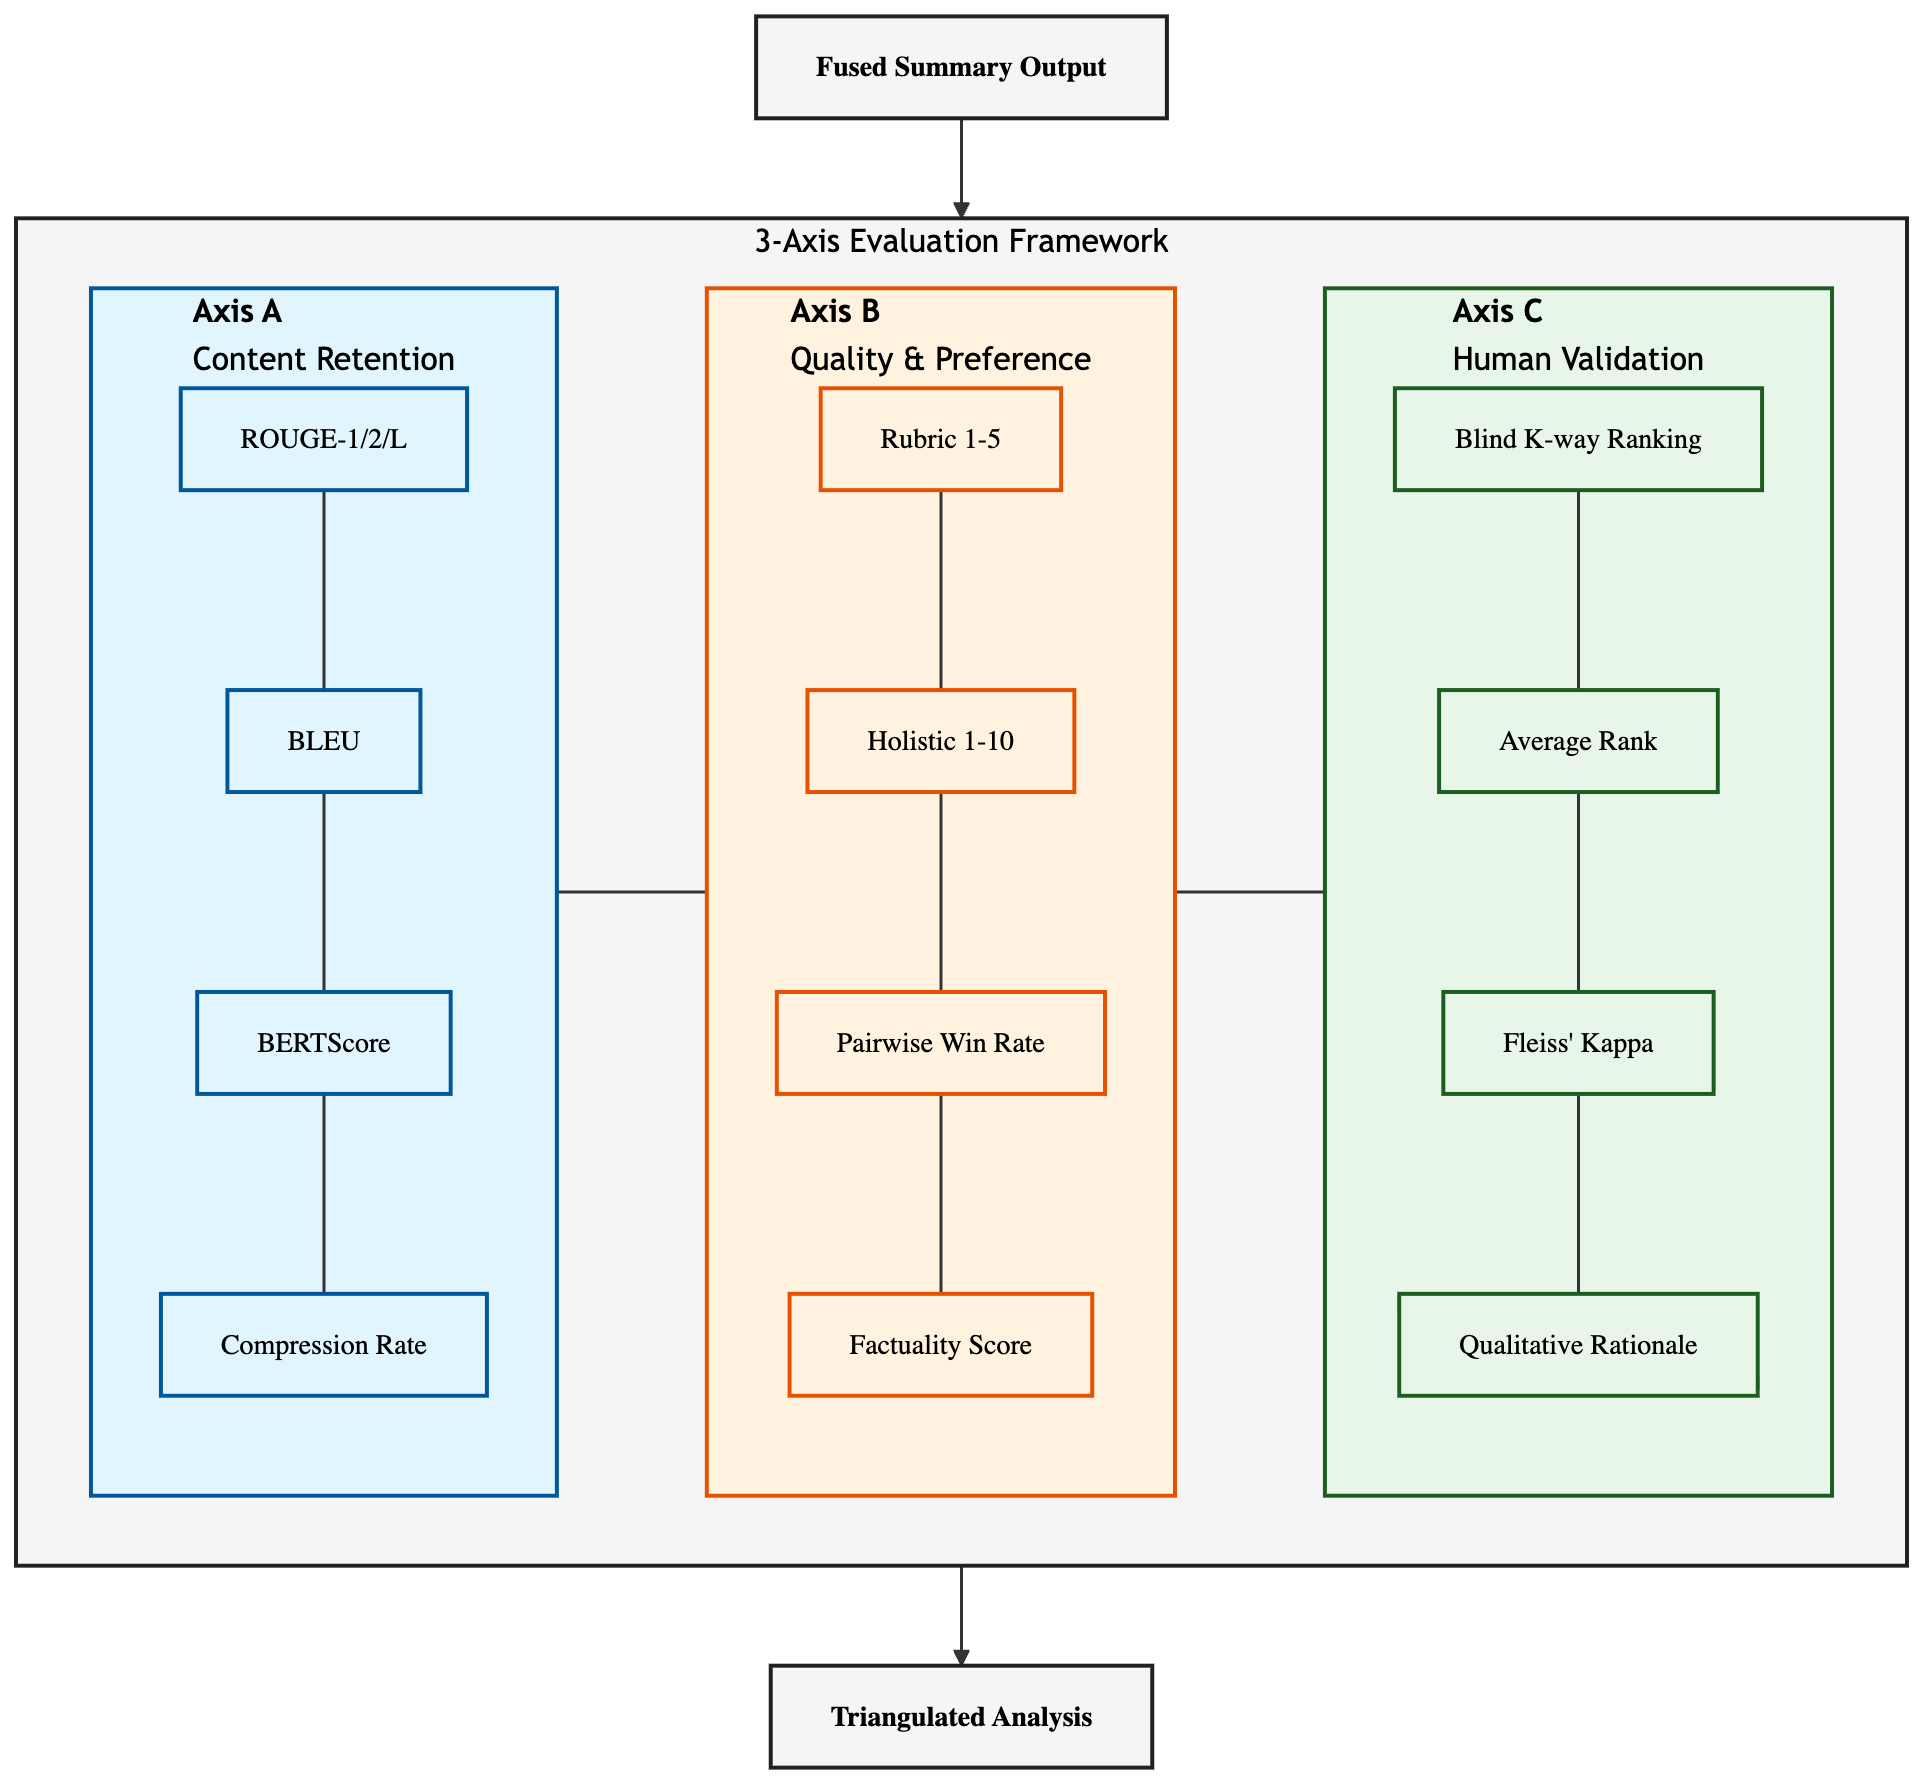
\includegraphics[width=0.9\linewidth]{figures/3-axis_framework.png}
  \caption{Khung đánh giá ba trục được sử dụng để định vị đa chiều chất lượng hệ thống.}
  \label{fig:evaluation_framework}
\end{figure}

\subsection{Trục A --- Khả năng giữ lại nội dung (Content Retention)}

Các số liệu thuộc Trục~A được tính toán tự động trong mô-đun 
\url{backend/services/evaluation.service.ts} ngay sau khi mỗi bản tóm tắt được tạo ra. 
Chỉ số ROUGE-1/2/L và BLEU được thực hiện thông qua các thư viện chuyển đổi JavaScript tương đương của \url{rouge} và \url{sacrebleu}. 
Chỉ số BERTScore được giao phó tính toán cho microservice viết bằng Python (\url{bert.service.ts}). 
Cả bốn chỉ số đánh giá chất lượng này đều được tính toán đối chiếu trực tiếp với \textit{văn bản bài viết gốc}, thay vì so sánh với bản tóm tắt mẫu do con người viết; 
đây là một điểm cần chú ý về mặt phương pháp luận (methodology caveat) được ghi chép rõ ràng trong báo cáo tổng hợp. Tỷ lệ nén được tính bằng công thức ký tự $|S|/|D|$.

\begin{figure}[H]
  \centering
  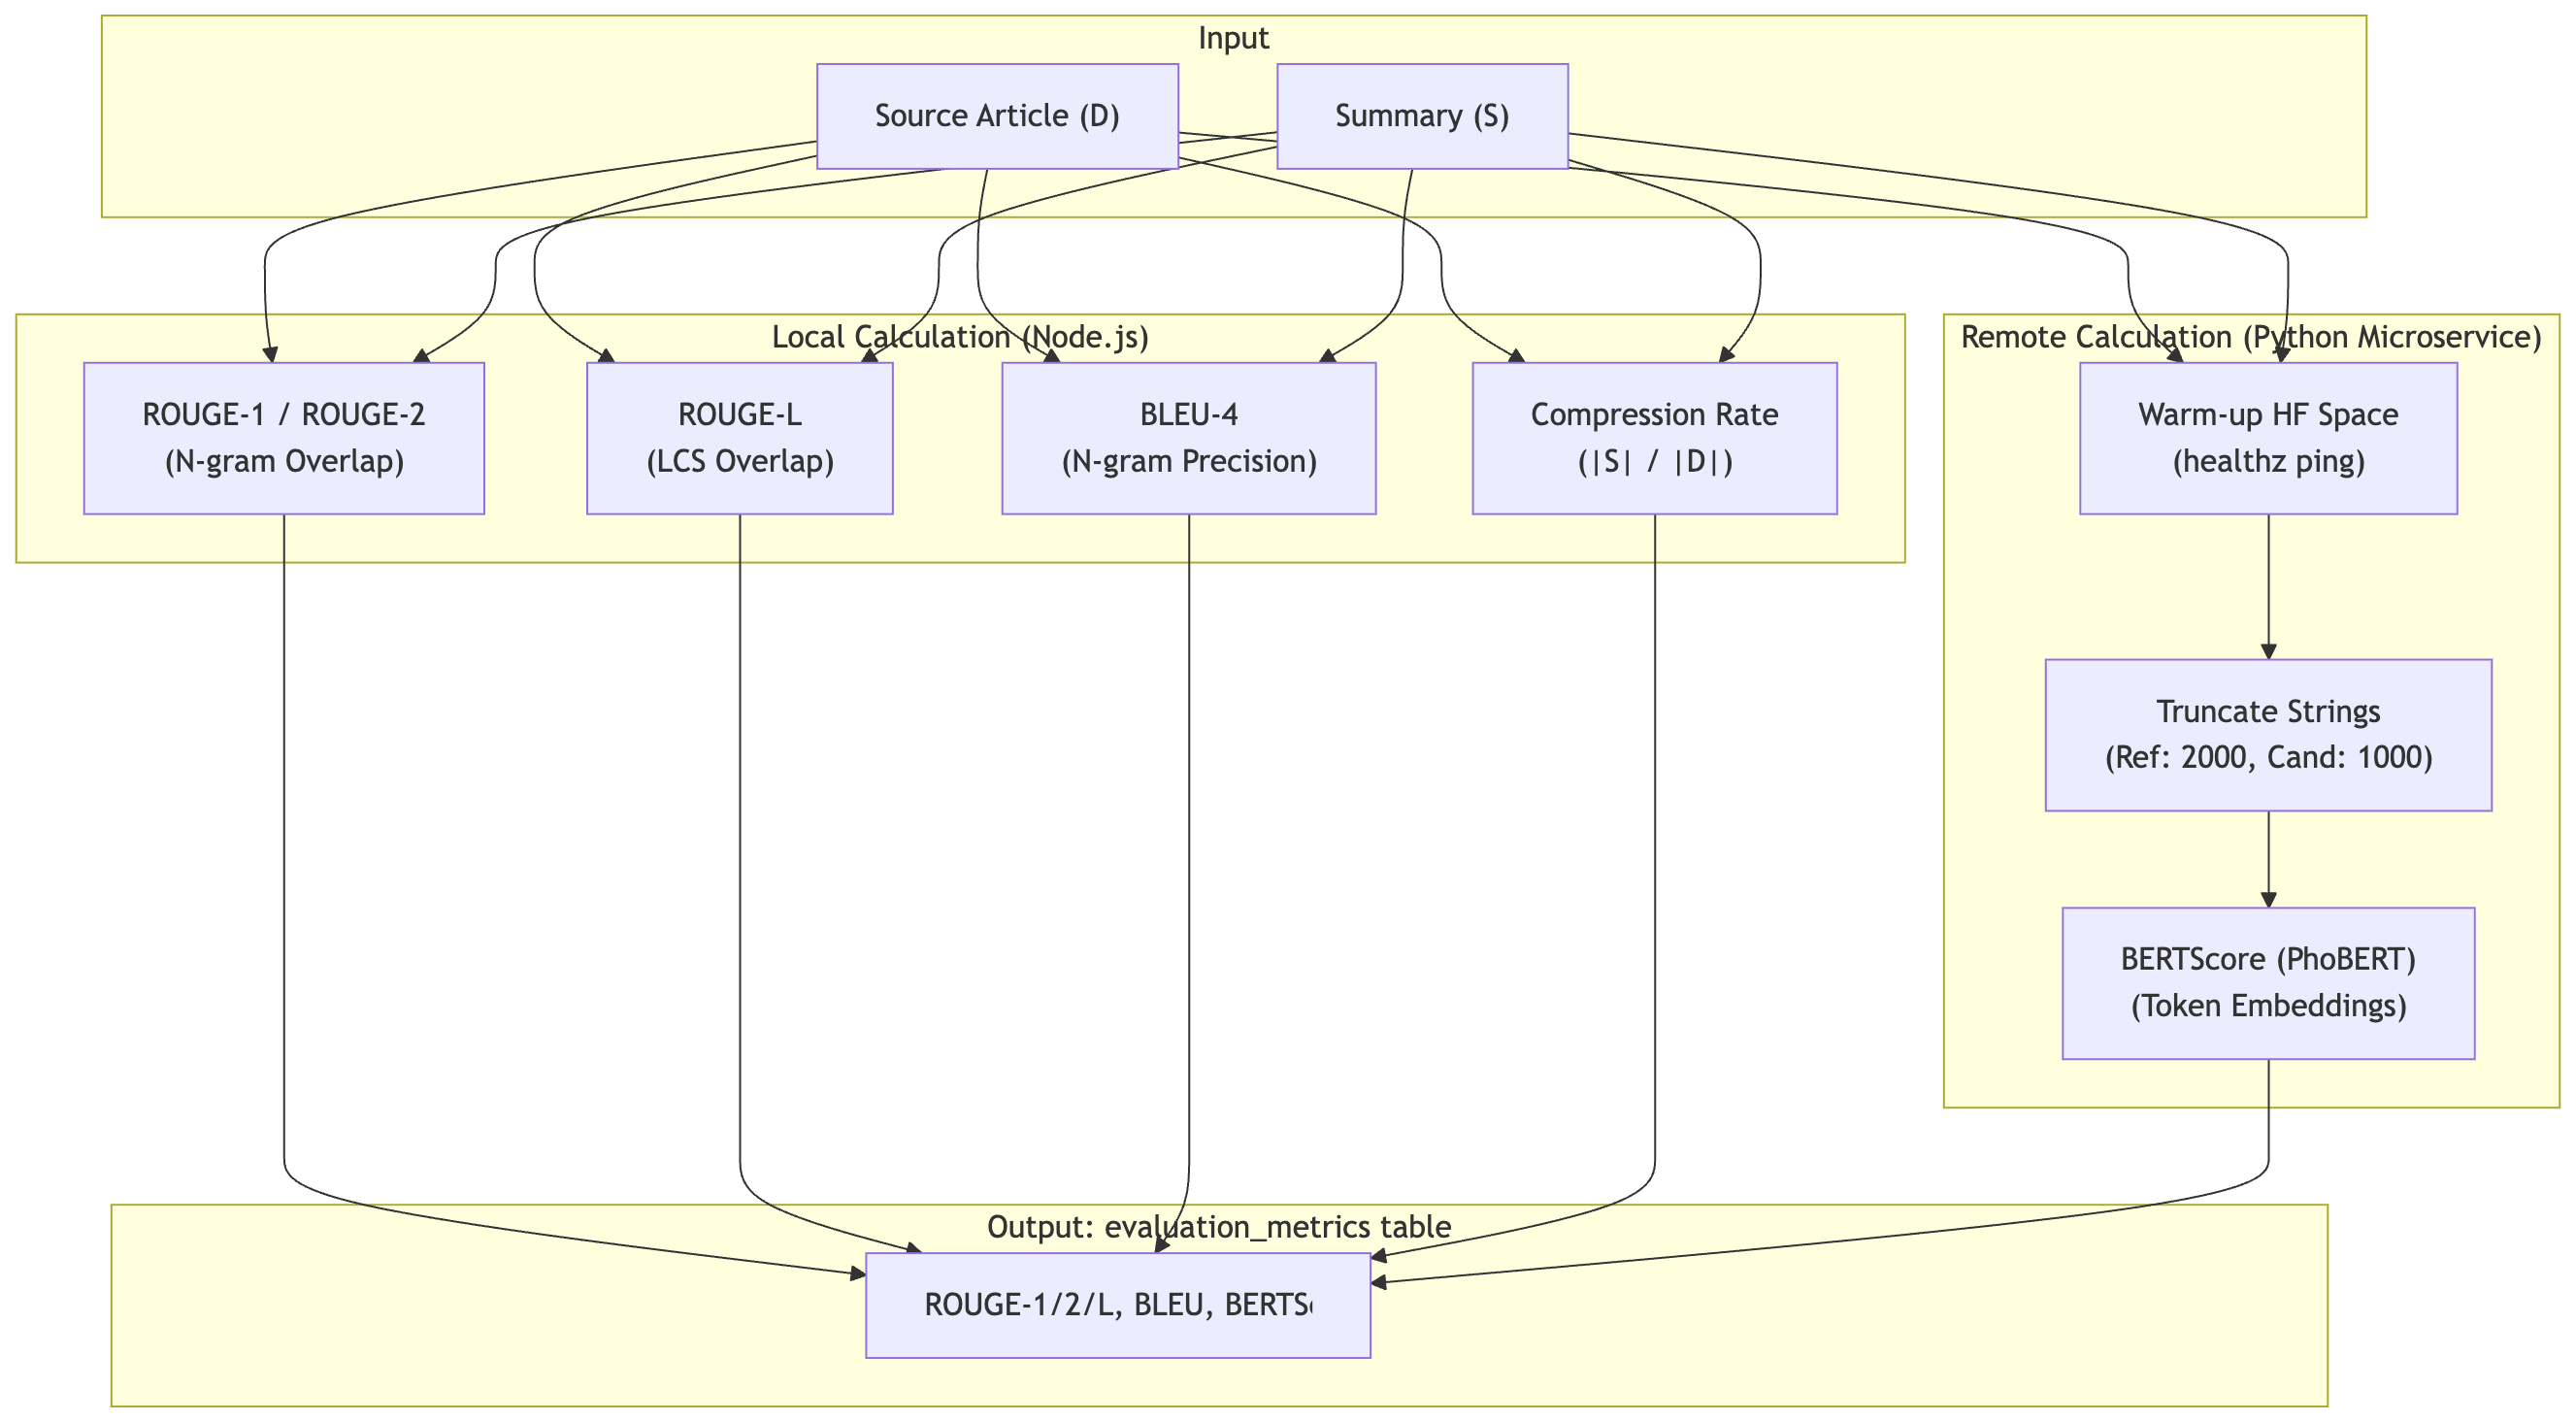
\includegraphics[width=\linewidth]{figures/A_calculation.png}
  \caption{Sơ đồ luồng tính toán các chỉ số thuộc Trục A (Khả năng giữ lại nội dung).}
  \label{fig:axis_a_calc}
\end{figure}

\subsection{Trục B --- Chất lượng và Sự ưu tiên (Quality and Preference)}

Trục~B đóng vai trò là trục trọng tâm của khóa luận. Mô-đun 
\url{llm-judge.service.ts} cung cấp bốn hàm chức năng chính:

\begin{itemize}
  \item \url{judgeRubric} --- Bộ tiêu chuẩn đánh giá 5 chiều phát triển từ FLASK trên thang điểm từ 1--5.
  \item \url{judgeAbsolute} --- Điểm số đánh giá toàn diện trên thang điểm 1--10 theo phong cách MT-Bench.
  \item \url{judgePairwise} --- Đánh giá so sánh cặp A so với B tích hợp cơ chế ngẫu nhiên hóa vị trí (position randomization).
  \item \url{scoreFactuality} (nằm trong \url{factuality.service.ts}) --- Phân tách tuyên bố kết hợp phân loại kéo theo logic (entailment classification).
\end{itemize}

Hai quy trình cấp cao hơn được vận hành riêng cho đầu ra của pipeline dung hợp MoA:

\begin{itemize}
  \item \url{runFusionPairwiseJudge} --- So sánh bản dịch dung hợp với bản thảo tốt nhất của tác nhân đề xuất (\url{comparison_type} = \url{vs_best_draft}).
  \item \url{runFusionVsAllDraftsJudge} --- So sánh bản dịch dung hợp với từng bản thảo đề xuất đơn lẻ (\url{comparison_type} = \url{vs_individual_draft}).
  \item Phép so sánh thứ ba, ``dung hợp MoA so với bản tóm tắt chạy trực tiếp trên \texttt{gpt-4o} đơn lẻ'' (\url{vs_single_aggregator}), được tạo ra bằng một tập kịch bản ngoại tuyến được mô tả tại Mục~4.3.2; đây là phép so sánh mang tính chất quyết định đối với toàn bộ khóa luận vì cả hai đối tượng so sánh đều là sản phẩm đầu ra của cùng một mô hình \texttt{gpt-4o}, nhờ đó triệt tiêu hoàn toàn thiên kiến tự ưu ái cùng họ mô hình của giám khảo LLM.
\end{itemize}

\begin{figure}[H]
  \centering
  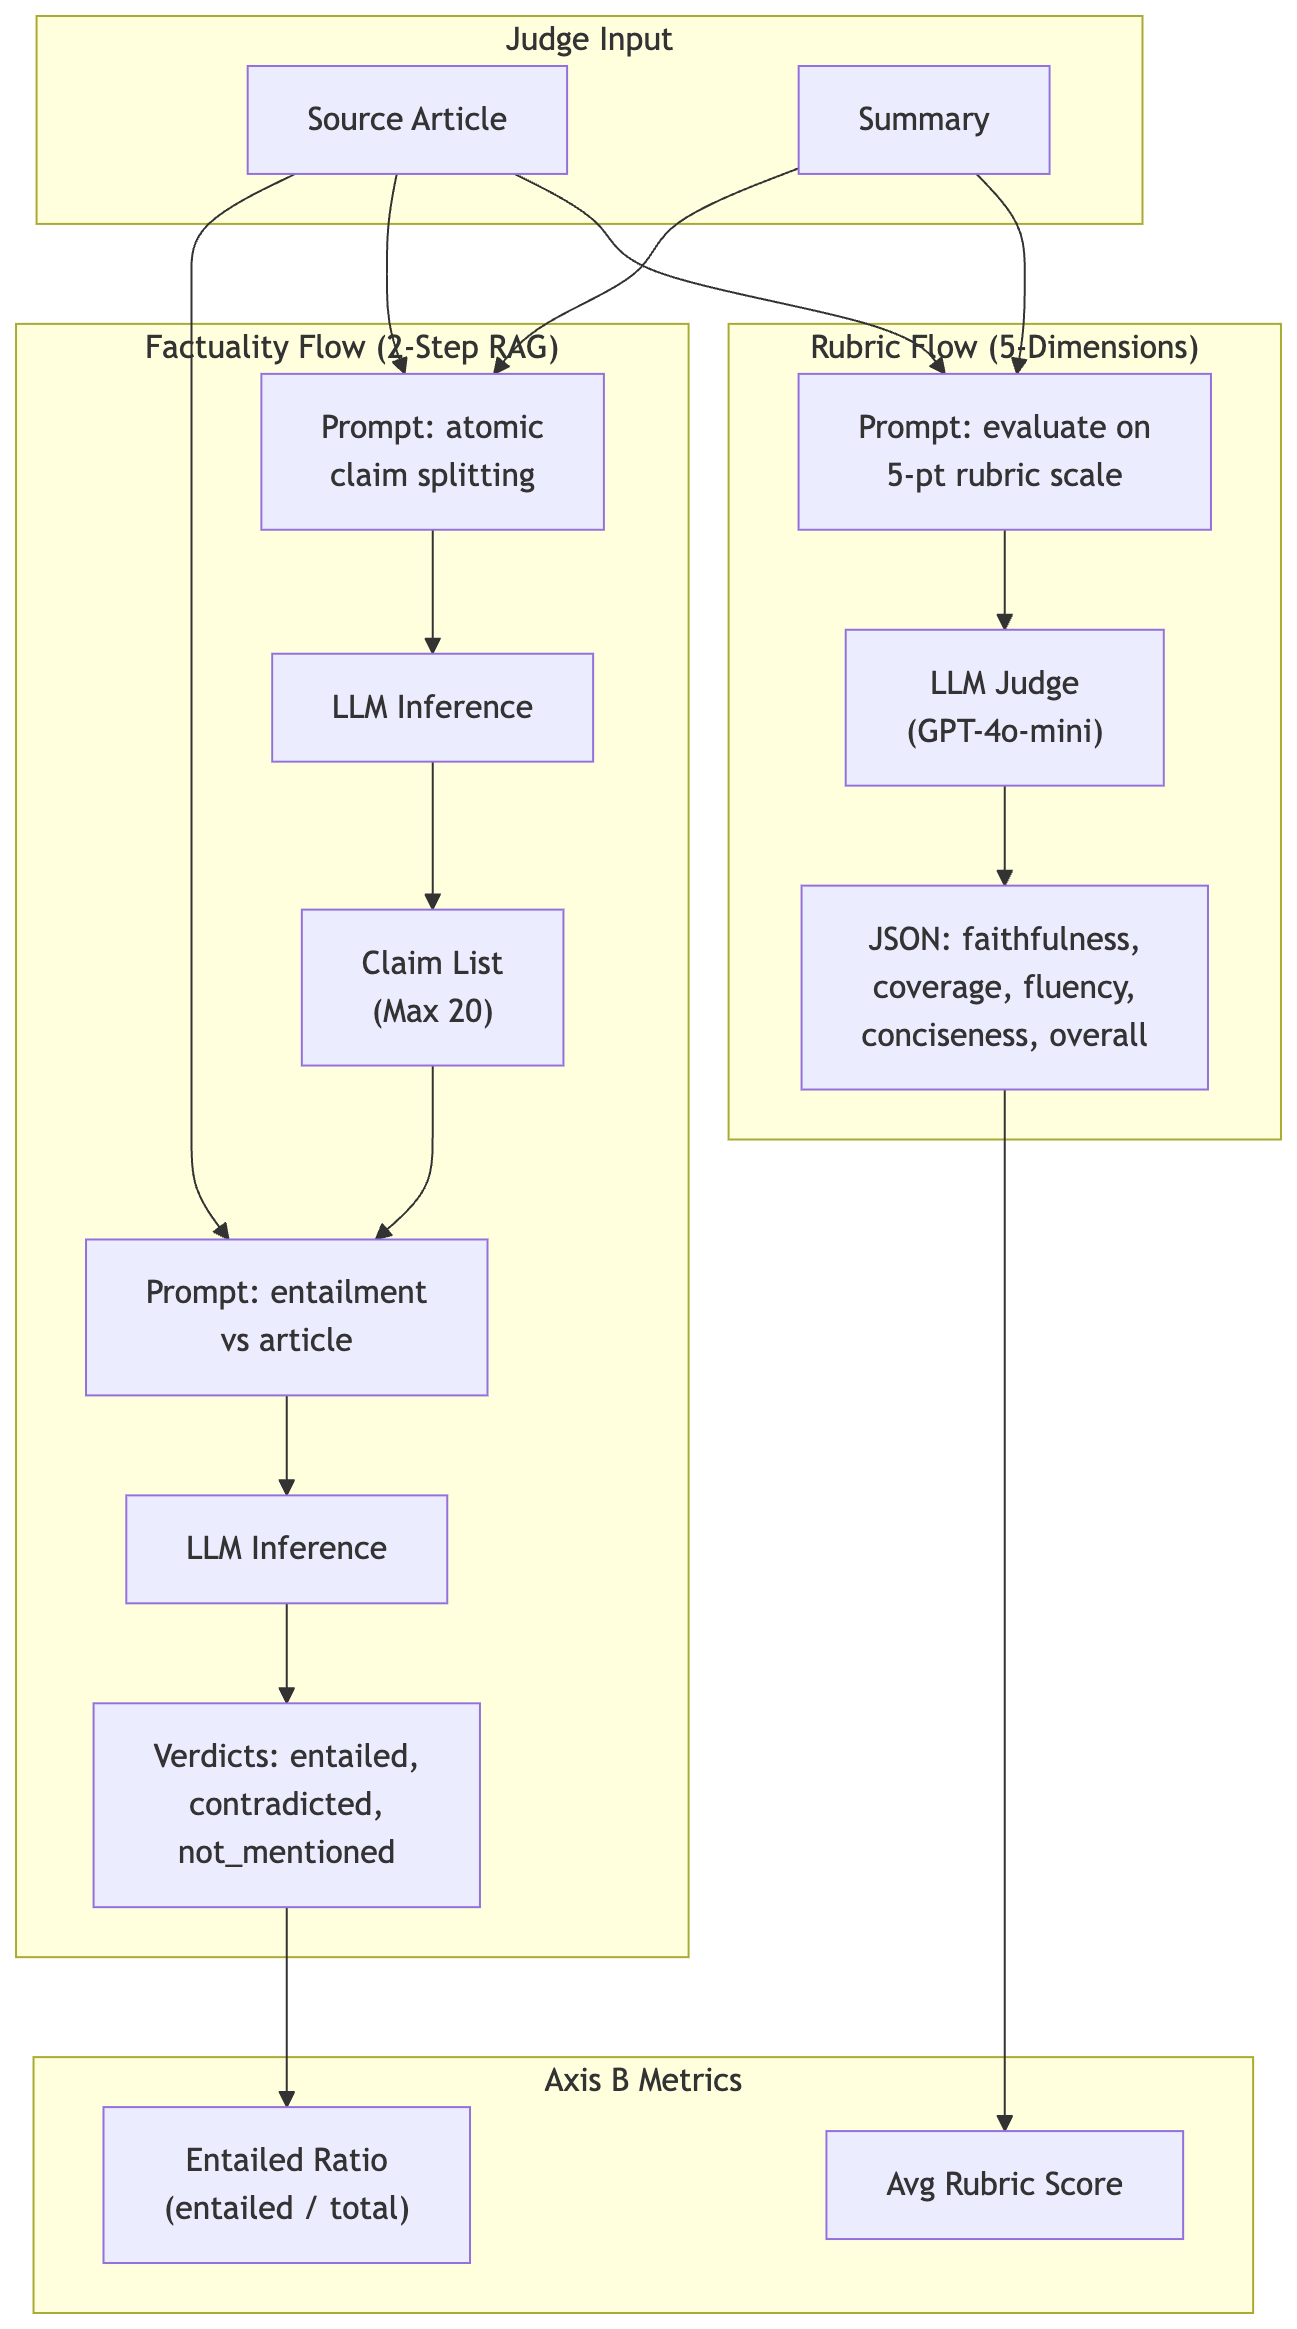
\includegraphics[height=0.6\textheight,keepaspectratio]{figures/B_calculation.png}
  \caption{Sơ đồ luồng xử lý đánh giá bằng giám khảo LLM thuộc Trục B (Chất lượng và Sự ưu tiên).}
  \label{fig:axis_b_calc}
\end{figure}

\subsection{Trục C --- Đánh giá con người (Human Validation)}

Trục~C sử dụng chính giao diện web của hệ thống để tổ chức các tác vụ xếp hạng mù dành cho người đánh giá.

\begin{itemize}
  \item Nhà nghiên cứu tạo một tác vụ đánh giá tại đường dẫn quản trị \texttt{/evaluate/admin}. Mỗi tác vụ tương ứng với một bài báo gốc và ba bản tóm tắt ứng viên (bản dịch dung hợp MoA, bản tóm tắt GPT-4o đơn lẻ, và bản thảo GPT-4o-mini) với danh tính mô hình đã được ẩn giấu hoàn toàn. Các ứng viên được gán nhãn trung lập là \textit{Bản A, Bản B, Bản C}.
  \item Người đánh giá truy cập đường dẫn \texttt{/evaluate?task=<uuid>}, nhập mã nhận diện định danh duy nhất (rater code), thực hiện thao tác kéo thả để xếp hạng vị trí của ba ứng viên, và viết một câu nhận xét ngắn bằng tiếng Việt giải thích lý do lựa chọn cho mỗi bản tóm tắt.
  \item Các phản hồi được ghi nhận vào bảng cơ sở dữ liệu \url{human_eval_responses}; một chỉ mục duy nhất một phần được thiết lập trên tổ hợp trường \url{(task_id, rater_id)} để ngăn chặn hành vi gửi phản hồi hai lần của cùng một người đánh giá trên một tác vụ.
  \item API \url{/api/human-eval/report} chịu trách nhiệm tính toán tổng hợp thứ hạng trung bình của từng mô hình, tỷ lệ thắng tương ứng, và hệ số độ đồng thuận Fleiss'~$\kappa$.
\end{itemize}

\begin{figure}[H]
  \centering
  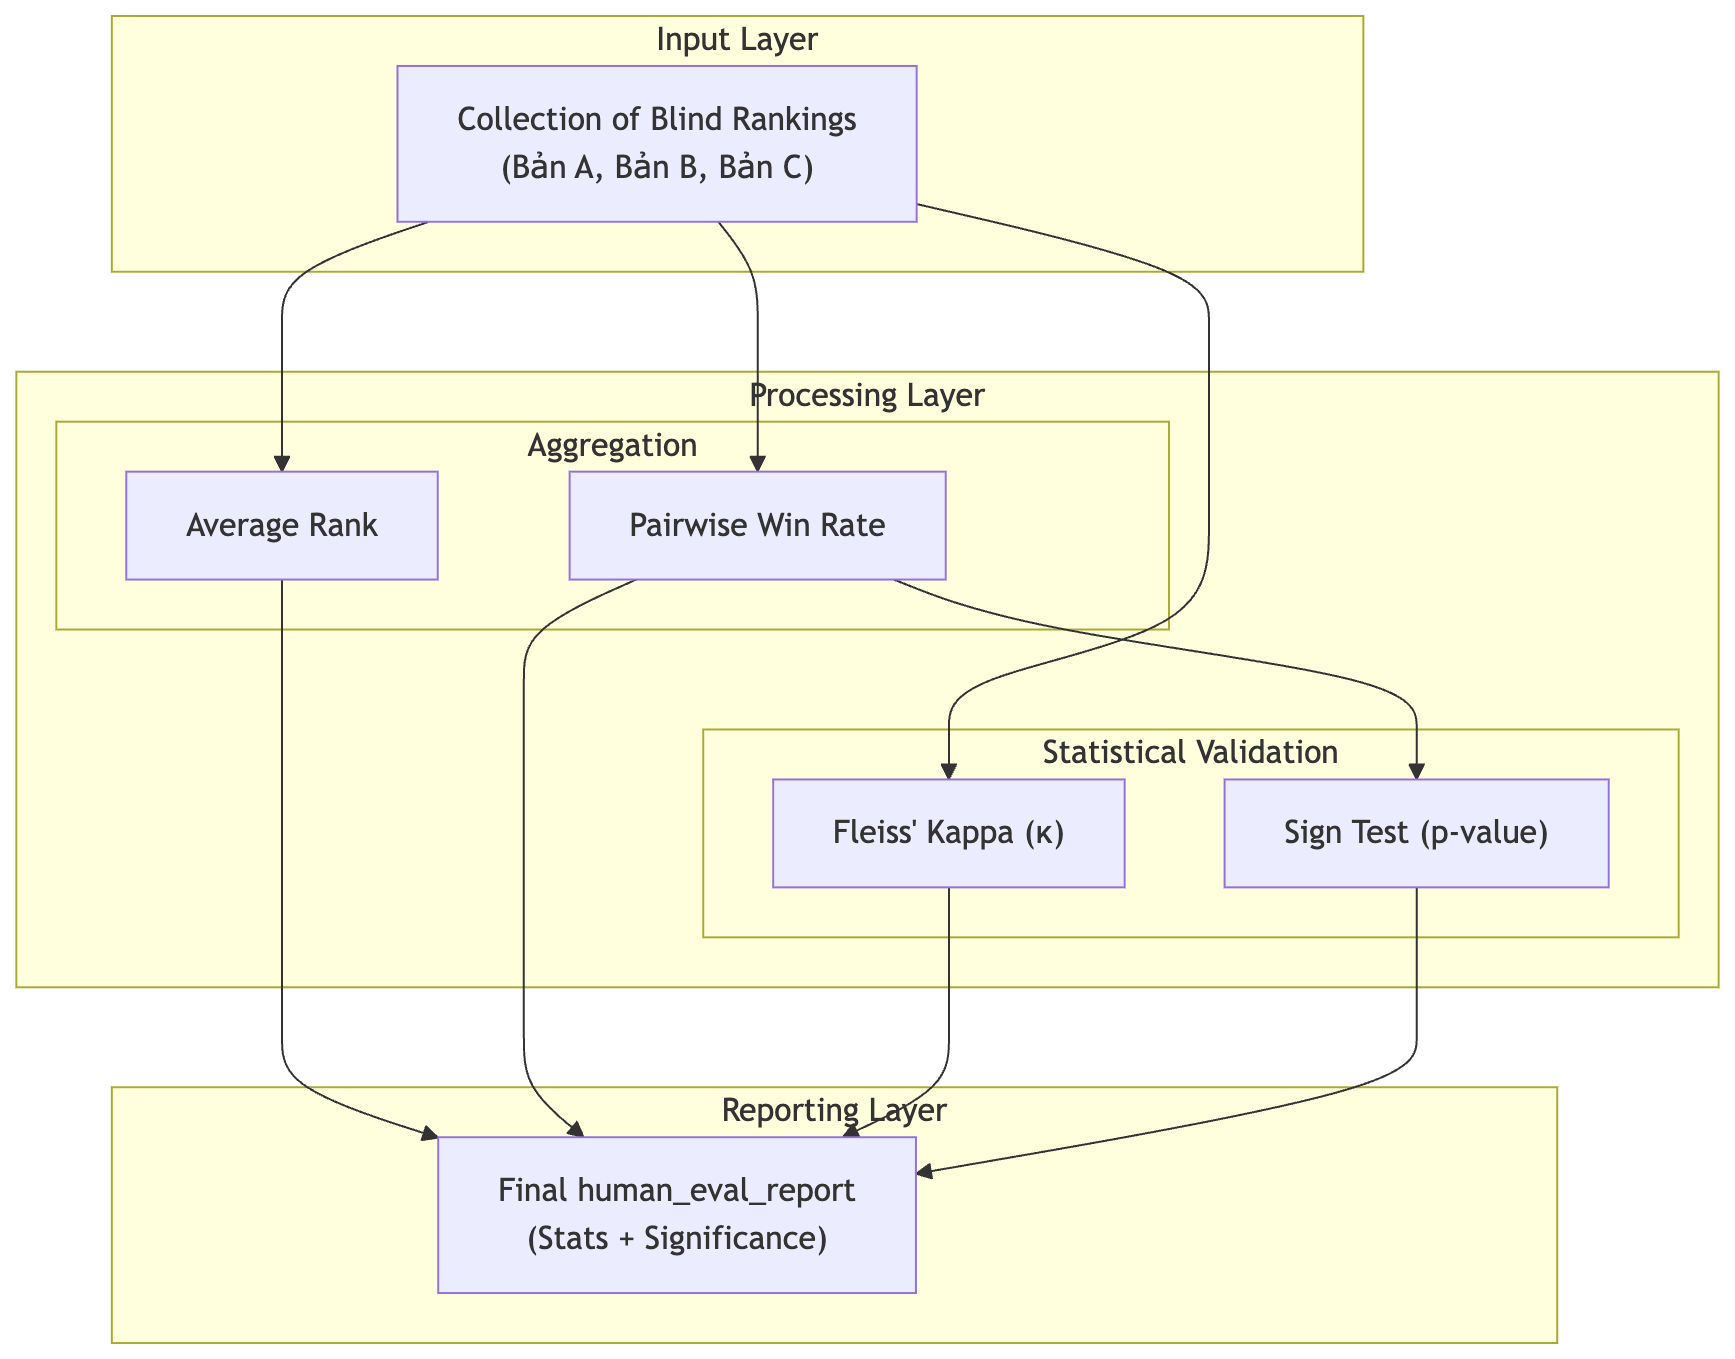
\includegraphics[width=\linewidth]{figures/C_calculation.png}
  \caption{Sơ đồ luồng xử lý và tổng hợp số liệu thống kê thuộc Trục C (Đánh giá con người).}
  \label{fig:axis_c_calc}
\end{figure}

\subsection{Phân tích thống kê}

Để đảm bảo các kết quả thực nghiệm thu được đạt độ tin cậy khoa học cao nhất, hệ thống tích hợp một thư viện xử lý thống kê chuyên biệt (\texttt{backend/}\allowbreak\texttt{output-fusion/}\allowbreak\texttt{scripts/}\allowbreak\texttt{stats.ts}). 
Quá trình triển khai tập trung xử lý bốn nhóm tác vụ cốt lõi nhằm đảm bảo các số liệu đo lường được báo cáo trong các chương tiếp theo đạt tính chính xác và khả năng tái lập cao:

\begin{itemize}
  \item \textbf{Kiểm định ý nghĩa thống kê (Trục A/B):} Hệ thống sử dụng phương pháp tính giá trị p-value nhị thức hai phía chính xác thông qua hàm \texttt{signTestPValue} để xác định xem khoảng cách hiệu năng giữa các mô hình có thực sự có ý nghĩa hay không. Để xử lý các bài toán có kích thước mẫu thực nghiệm lớn mà không gây lỗi tràn số bộ nhớ, tôi đã thiết kế một \textit{bộ đệm lưu log-giai thừa (log-factorial cache)}. Kỹ thuật này giúp hệ thống thực hiện các phép tính trong không gian logarit, triệt tiêu hoàn toàn hiện tượng tràn số dấu phẩy động thường gặp khi tính toán các tổ hợp lớn $C(n, k)$.
  \item \textbf{Hiệu chỉnh thiên kiến độ dài (Trục B):} Do các mô hình ngôn ngữ lớn làm giám khảo thường có xu hướng ưu tiên các văn bản đầu ra có độ dài lớn hơn \cite{Dubois2024}, tôi đã triển khai giải thuật \texttt{length}\allowbreak\texttt{Bucketed}\allowbreak\texttt{WinRate}. Bằng cách phân chia các phán quyết vào ba nhóm (buckets) dựa trên tỷ lệ độ dài tương ứng $L_{\text{A}}/L_{\text{B}}$ ($<0.85$, $0.85$--$1.15$, và $>1.15$), hệ thống có thể tính toán một tỷ lệ thắng cân bằng và khách quan hơn, không còn bị chi phối bởi xu hướng "thích bài dài" của mô hình.
  \item \textbf{Độ đồng thuận giữa các người đánh giá (Trục C):} Để đo lường mức độ thống nhất trong các quyết định xếp hạng của những người đánh giá con người độc lập, hệ thống tính toán hệ số Fleiss' $\kappa$ thông qua hàm \texttt{fleiss}\allowbreak\texttt{Kappa}\allowbreak\texttt{From}\allowbreak\texttt{Rankings}. Tôi áp dụng bộ khung diễn giải tiêu chuẩn của Landis và Koch \cite{Landis1977} để đánh giá các chỉ số này, hướng tới việc đạt hệ số đồng thuận ở mức ít nhất là "trung bình" ($\kappa > 0.4$) để đảm bảo nghiên cứu khảo sát con người đạt độ giá trị khoa học cần thiết.
  \item \textbf{Tổng hợp số liệu cặp (Paired Metric Aggregation):} Đối với các chỉ số đo lường khả năng giữ lại nội dung ở Trục A, hàm \texttt{paired}\allowbreak\texttt{Metric}\allowbreak\texttt{Stats} chịu trách nhiệm tự động tính toán giá trị trung bình, độ lệch chuẩn và sai lệch cặp thực nghiệm. Giải thuật được thiết kế để tự động loại bỏ các dữ liệu khuyết thiếu (missing data) và tính toán p-value kiểm định dấu (sign-test) cho các phép so sánh đối đầu trực tiếp, cung cấp một phương thức chuẩn hóa để báo cáo số liệu trên toàn bộ Trục A.
\end{itemize}

\subsection{Dung hợp MoA so với GPT-4o đơn lẻ (Thesis-Decisive)}

Phép so sánh mang tính chất quyết định này loại bỏ hoàn toàn một yếu tố gây nhiễu (confound) thường xuất hiện trong các so sánh giữa bản dịch dung hợp và bản thảo đề xuất \textit{tốt nhất}: 
bản thảo đề xuất tốt nhất vốn được tạo ra bởi một mô hình có năng lực yếu hơn tác nhân tổng hợp, do đó bất kỳ chiến thắng nào của bản dịch dung hợp cũng có thể bị quy kết một cách phiến diện là do ``GPT-4o mạnh hơn Claude Haiku''. 
Bằng cách so sánh trực tiếp bản dịch dung hợp MoA (sử dụng GPT-4o làm tác nhân tổng hợp) chống lại chính mô hình GPT-4o chạy độc lập ở chế độ không dữ liệu mẫu (zero-shot) trên cùng một bài báo gốc, cả hai ứng viên so tài đều là sản phẩm đầu ra của cùng một mô hình GPT-4o. 
Do đó, bất kỳ sự vượt trội nào ghi nhận được cũng chỉ có thể được giải thích một cách duy nhất là do hiệu quả của quá trình \textit{dung hợp và tổng hợp thông tin} — khi tác nhân tổng hợp được cung cấp thêm ngữ cảnh là nhiều bản thảo đề xuất đa dạng từ các họ mô hình khác nhau — chứ không phải do sự chênh lệch về năng lực cốt lõi của bản thân mô hình nền tảng. 
Quy trình thực nghiệm này được triển khai thông qua các tệp kịch bản \texttt{scripts/run-single-baseline.ts} và \texttt{scripts/compare-fused-vs-single.ts}; toàn bộ các kết quả thực nghiệm chi tiết sẽ được trình bày tại Mục~4.3.2.

\section{Thiết kế cơ sở dữ liệu}

Cơ sở dữ liệu PostgreSQL trên nền tảng Supabase được tổ chức thông qua hai mươi lăm tệp di trú cấu trúc (migrations). 
Lược đồ cơ sở dữ liệu (schema) được phân chia mạch lạc thành ba nhóm chức năng chính: các số liệu đo lường chất lượng trên mỗi lượt tóm tắt, dữ liệu đặc thù phục vụ cấu trúc MoA, và hồ sơ lưu trữ các tác vụ đánh giá con người. 
Các mối liên kết logic giữa ba nhóm chức năng này được minh họa chi tiết thông qua sơ đồ Thực thể - Quan hệ (ER) trong Hình~\ref{fig:database_schema}.

\begin{figure}[H]
  \centering
  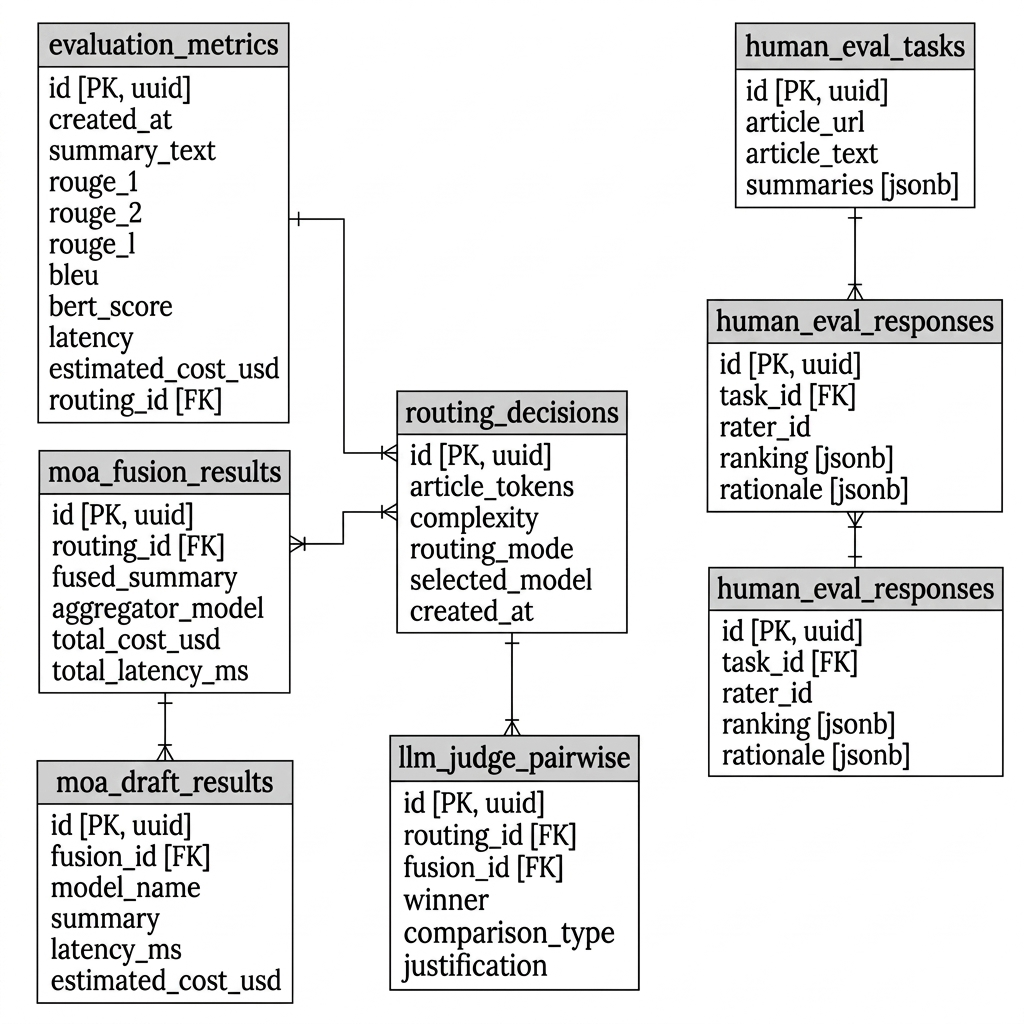
\includegraphics[width=\linewidth]{figures/database_schema.png}
  \caption{Lược đồ cơ sở dữ liệu Fiber (Supabase PostgreSQL) mô tả các bảng chính và mối quan hệ giữa chúng.}
  \label{fig:database_schema}
\end{figure}

\subsection{Các chỉ số đo lường trên từng bản tóm tắt và quyết định định tuyến}

Nhóm bảng này chịu trách nhiệm theo dõi toàn bộ vòng đời của mỗi yêu cầu tóm tắt gửi tới hệ thống, bắt đầu từ logic định tuyến ban đầu cho đến các kết quả đo lường chất lượng được tính toán sau đó.

\begin{table}[H]
\centering
\caption{Lược đồ cho các bảng \texttt{evaluation\_metrics} và \texttt{routing\_decisions}.}
\begin{tabular}{lll}
\hline
\textbf{Bảng / Cột} & \textbf{Kiểu dữ liệu} & \textbf{Mô tả chi tiết} \\ \hline
\textit{evaluation\_metrics} & & \\
\texttt{summary\_text} & text & Nội dung chi tiết của bản tóm tắt được tạo ra. \\
\texttt{rouge\_1/2/L} & float8 & Trục A: Điểm số ROUGE F1-score tương ứng. \\
\texttt{bert\_score} & float8 & Trục A: Điểm số tương đồng ngữ nghĩa BERTScore. \\
\texttt{latency} & int4 & Tổng thời gian xử lý từ đầu đến cuối hệ thống (ms). \\
\texttt{judge\_rubric} & jsonb & Trục B: Kết quả đánh giá Rubric đa chiều dưới dạng JSON. \\
\texttt{factuality\_ratio} & numeric & Trục B: Tỷ lệ các tuyên bố được kéo theo logic từ nguồn. \\ \hline
\textit{routing\_decisions} & & \\
\texttt{article\_tokens} & int4 & Số lượng từ tố ước tính của văn bản đầu vào. \\
\texttt{complexity} & text & Mức độ phức tạp được phân loại (Thấp/Trung bình/Cao). \\
\texttt{routing\_mode} & text & Chế độ định tuyến hiện hoạt (auto, forced, hoặc fusion). \\
\texttt{selected\_model} & text & Mô hình cụ thể được bộ định tuyến phân bổ xử lý. \\ \hline
\end{tabular}
\end{table}

\subsection{Cấu trúc dữ liệu đặc thù MoA}

Các bảng này chịu trách nhiệm lưu trữ các bản thảo sơ bộ ở lớp trung gian và kết quả dung hợp cuối cùng của pipeline đa tác nhân MoA, kết hợp cùng các phán quyết đánh giá so sánh cặp của giám khảo LLM.

\begin{table}[H]
\centering
\caption{Lược đồ cho các bảng đặc thù phục vụ cấu trúc MoA.}
\begin{tabular}{lll}
\hline
\textbf{Bảng / Cột} & \textbf{Kiểu dữ liệu} & \textbf{Mô tả chi tiết} \\ \hline
\textit{moa\_fusion\_results} & & \\
\texttt{fused\_summary} & text & Bản tóm tắt dung hợp cuối cùng. \\
\texttt{aggregator\_model} & text & Tên mô hình tổng hợp được sử dụng (ví dụ: GPT-4o). \\
\texttt{total\_cost\_usd} & float4 & Tổng chi phí tích lũy của toàn bộ lượt gọi LLM trong phiên. \\ \hline
\textit{moa\_draft\_results} & & \\
\texttt{model\_name} & text & Tên nhận diện của mô hình đề xuất (proposer). \\
\texttt{summary} & text & Nội dung bản thảo sơ bộ được tạo bởi mô hình đề xuất tương ứng. \\ \hline
\textit{llm\_judge\_pairwise} & & \\
\texttt{winner} & text & Kết quả phán quyết so sánh cặp (Bản A, Bản B, hoặc Hòa - Tie). \\
\texttt{comparison\_type} & text & Loại so sánh (so với bản thảo tốt nhất, so với từng bản thảo lẻ, v.v.). \\
\texttt{justification} & text & Đoạn giải thích lý do phán quyết bằng ngôn ngữ tự nhiên của giám khảo. \\ \hline
\end{tabular}
\end{table}

\subsection{Hồ sơ đánh giá của con người}

Nhóm bảng cuối cùng này chịu trách nhiệm quản lý và lưu giữ thông tin liên quan đến các tác vụ xếp hạng mù dành cho những người tham gia đánh giá con người.

\begin{table}[H]
\centering
\caption{Lược đồ cho các bảng phục vụ đánh giá của con người.}
\begin{tabular}{lll}
\hline
\textbf{Bảng / Cột} & \textbf{Kiểu dữ liệu} & \textbf{Mô tả chi tiết} \\ \hline
\textit{human\_eval\_tasks} & & \\
\texttt{article\_url} & text & Đường dẫn URL bài báo gốc dùng làm tham chiếu. \\
\texttt{summaries} & jsonb & Danh sách các bản tóm tắt ứng viên đã ẩn danh mô hình. \\ \hline
\textit{human\_eval\_responses} & & \\
\texttt{ranking} & jsonb & Danh sách xếp hạng thứ tự ưu tiên do người đánh giá quyết định. \\
\texttt{rationale} & jsonb & Các nhận xét giải thích chi tiết cho từng bản tóm tắt tương ứng. \\ \hline
\end{tabular}
\end{table}

\section{Giao diện người dùng}

\subsection{Thanh bên của tiện ích mở rộng (Extension Sidebar)}

Thanh bên của tiện ích mở rộng là bề mặt tương tác chính của người dùng với hệ thống (Hình~\ref{fig:sidebar}). 
Khi nhấn vào biểu tượng của tiện ích trên thanh công cụ, một bảng điều khiển sẽ được nhúng trực tiếp vào mép phải của trang web hiện tại; bảng này được thiết kế chuyên biệt và tối giản hóa, chỉ hiển thị khu vực tóm tắt dạng luồng thời gian thực. 
Khác với giao diện popup hay các bảng điều khiển dạng hộp thoại khác, thanh bên này hoàn toàn không có thêm các nút bấm hay trình điều khiển phức tạp nào, đóng vai trò là một không gian đọc tập trung và tinh tế dành riêng cho bản tóm tắt tin tức.

\begin{figure}[H]
  \centering
  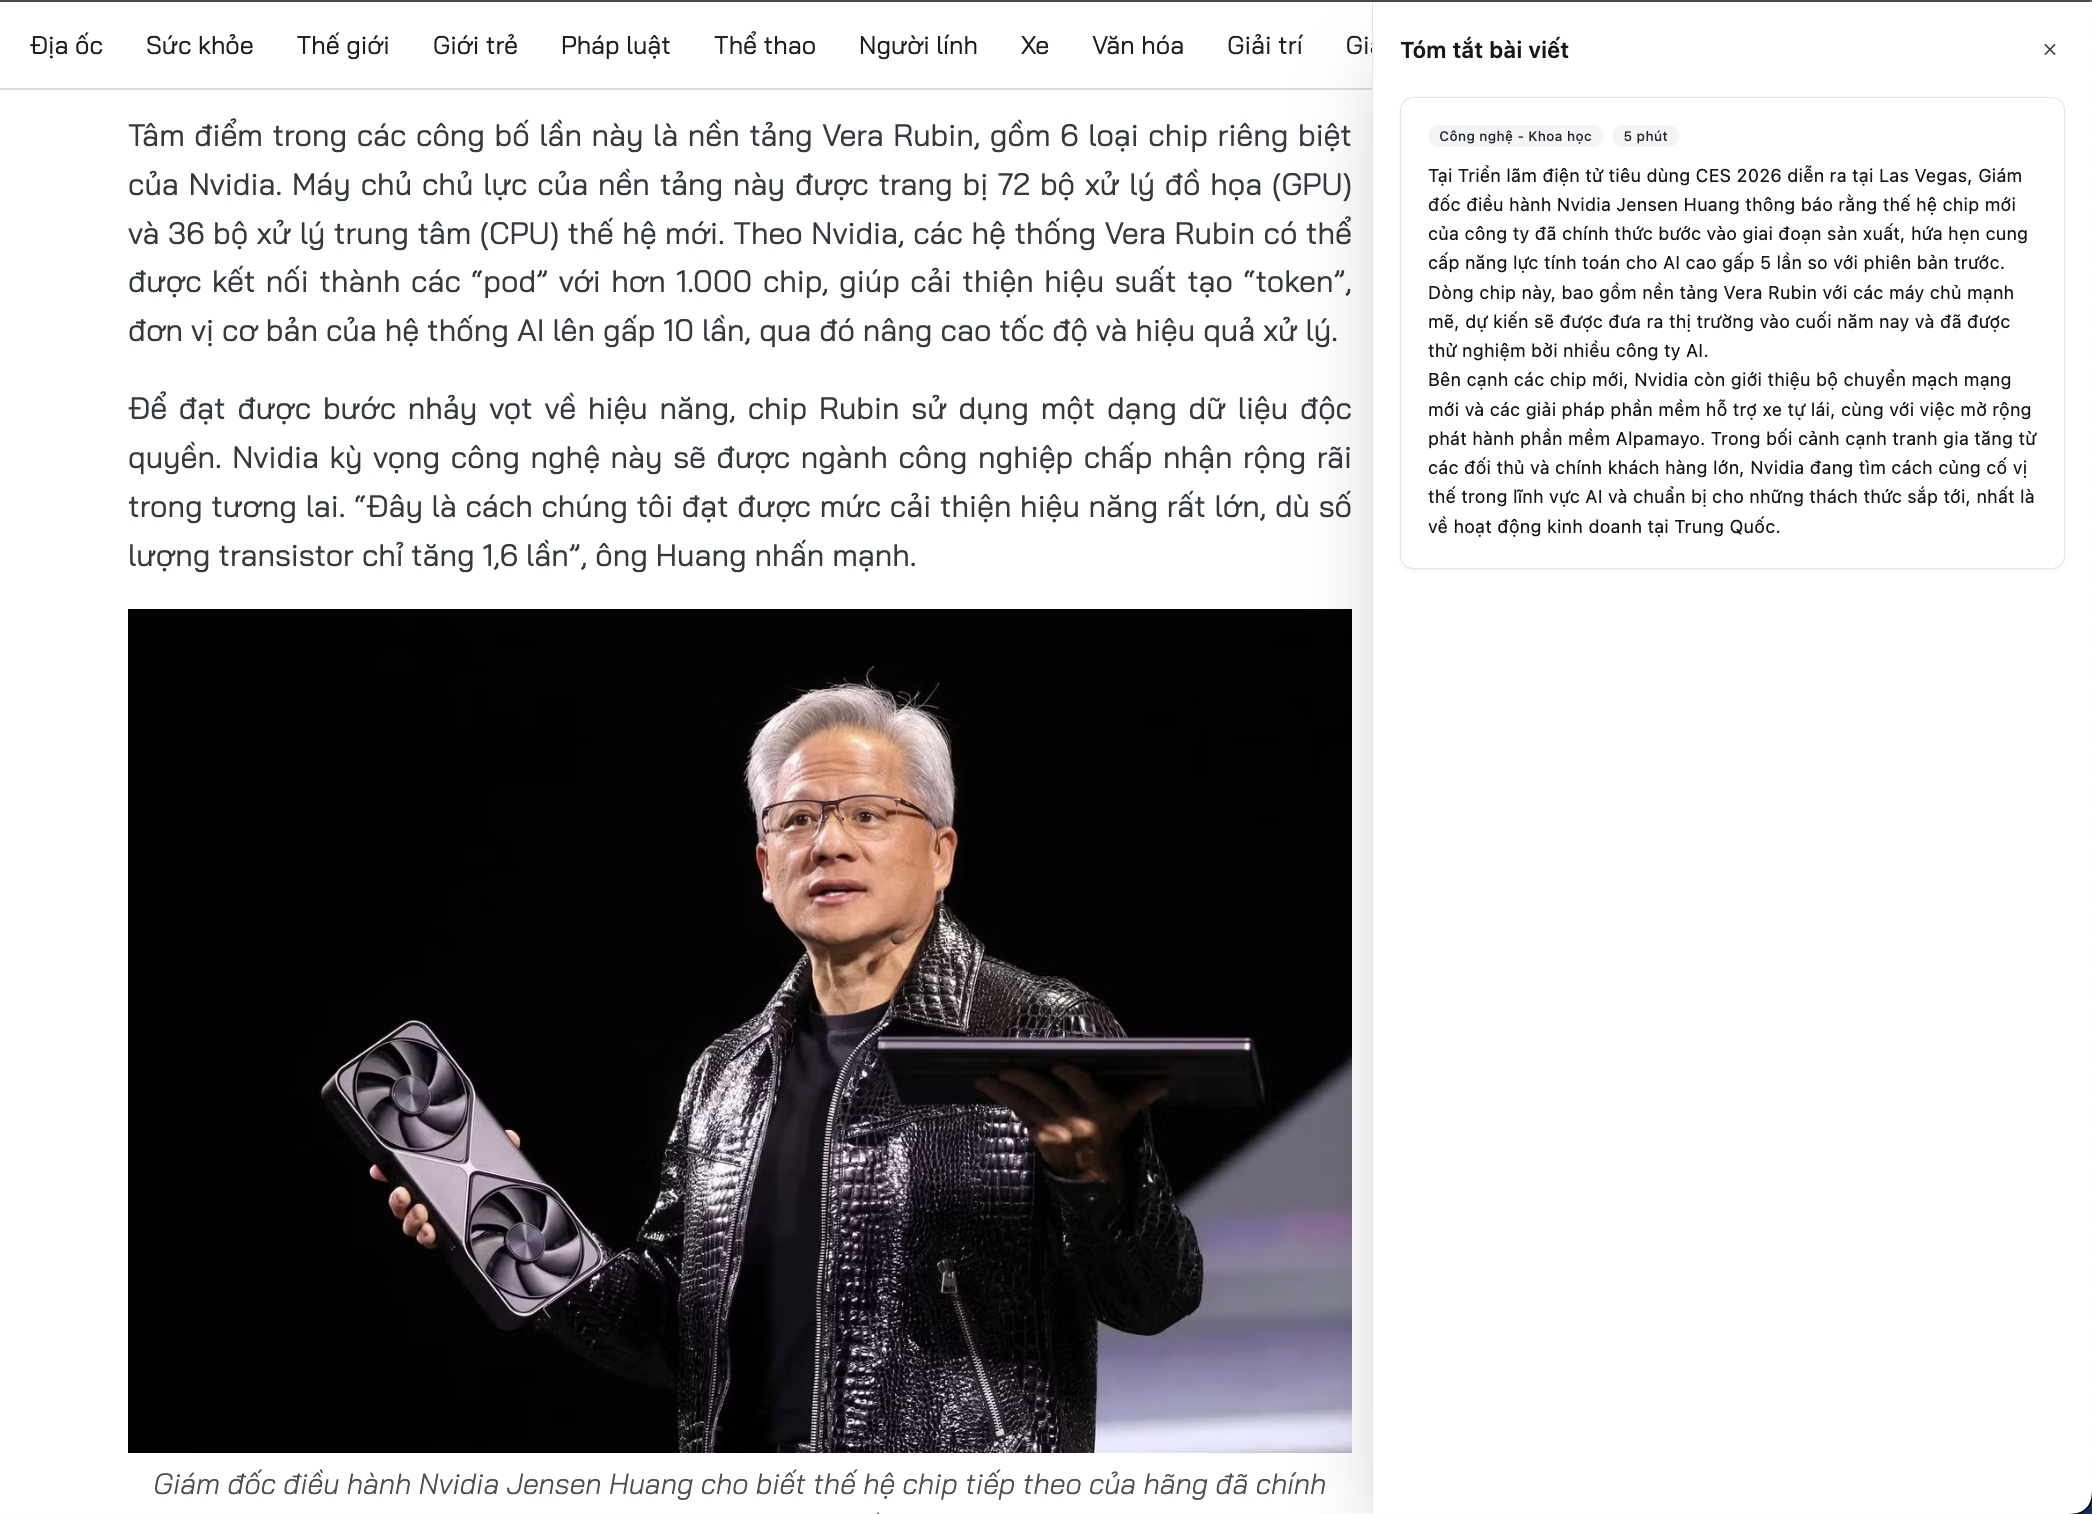
\includegraphics[width=0.85\linewidth]{figures/sidebar.png}
  \caption{Thanh bên của tiện ích mở rộng Fiber.}
  \label{fig:sidebar}
\end{figure}

\subsection{Khung hội thoại kiểm chứng (Fact-checking Modal)}

Khung hội thoại kiểm chứng (Hình~\ref{fig:fact_check_modal}) cung cấp một giao diện phân tích cực kỳ chi tiết về quy trình xác thực thông tin. 
Hệ thống tự động phân tách bản tóm tắt thành các tuyên bố nguyên tử độc lập và hiển thị mỗi tuyên bố kèm theo điểm số độ tin cậy và trạng thái phân loại màu sắc trực quan (màu xanh lá tương ứng với đã được xác thực, màu vàng tương ứng với xác thực một phần, và màu đỏ tương ứng với thông tin ảo tưởng). 
Người dùng có thể nhấn vào các đường dẫn nguồn minh chứng được liệt kê để đối chiếu và kiểm tra thông tin trực tiếp một cách nhanh chóng.

\begin{figure}[H]
  \centering
  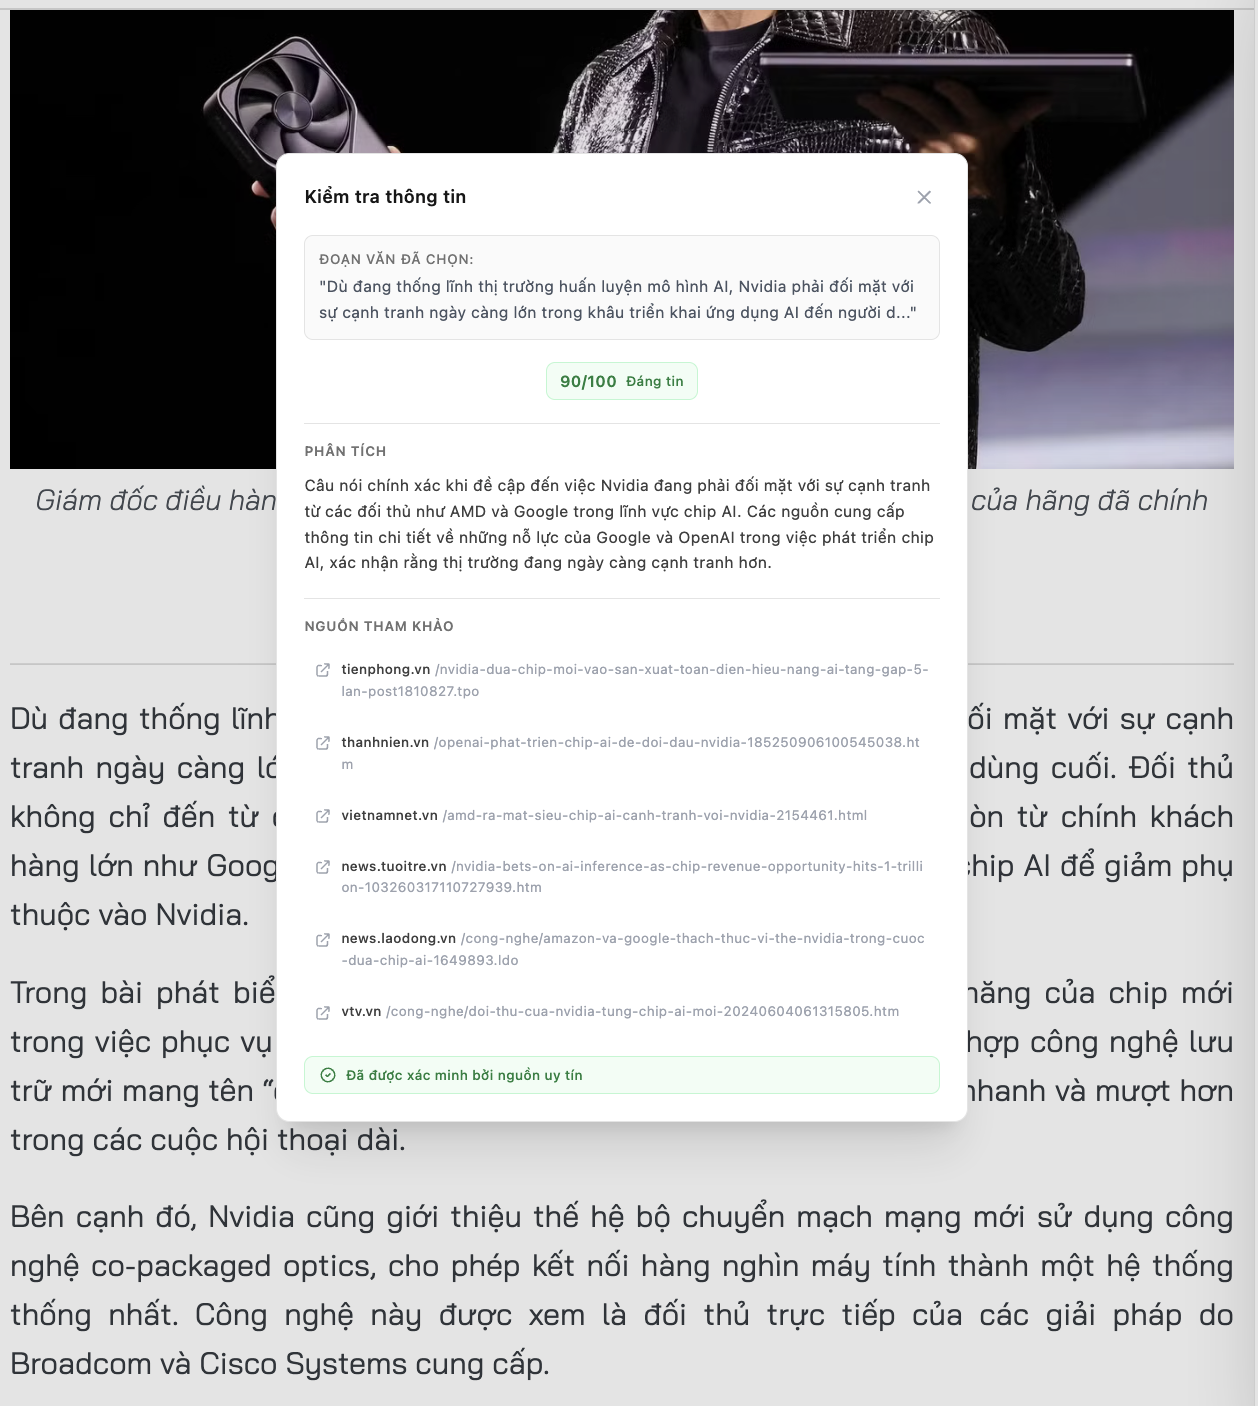
\includegraphics[width=0.85\linewidth]{figures/fact_check_modal.png}
  \caption{Khung hội thoại kiểm chứng hiển thị chi tiết các tuyên bố được xác thực.}
  \label{fig:fact_check_modal}
\end{figure}

\subsection{Trang số liệu đo lường (\texttt{/metrics})}

Trang báo cáo số liệu đo lường (Hình~\ref{fig:metrics_dashboard}) chịu trách nhiệm hiển thị toàn bộ nội dung của bảng \url{evaluation_metrics} 
thông qua hai chế độ xem linh hoạt (\textit{thu gọn - compact}, và \textit{đầy đủ - full}), tích hợp các bộ lọc tìm kiếm theo chế độ định tuyến và loại mô hình sử dụng. 
Trang được thiết kế trực quan với ba biểu đồ nhúng thời gian thực: biểu đồ radar năm trục thể hiện chất lượng Rubric, huy hiệu đánh giá so sánh cặp giữa MoA dung hợp so với bản thảo tốt nhất, và vòng tròn phân bổ tính xác thực kéo theo logic.

\begin{figure}[H]
  \centering
  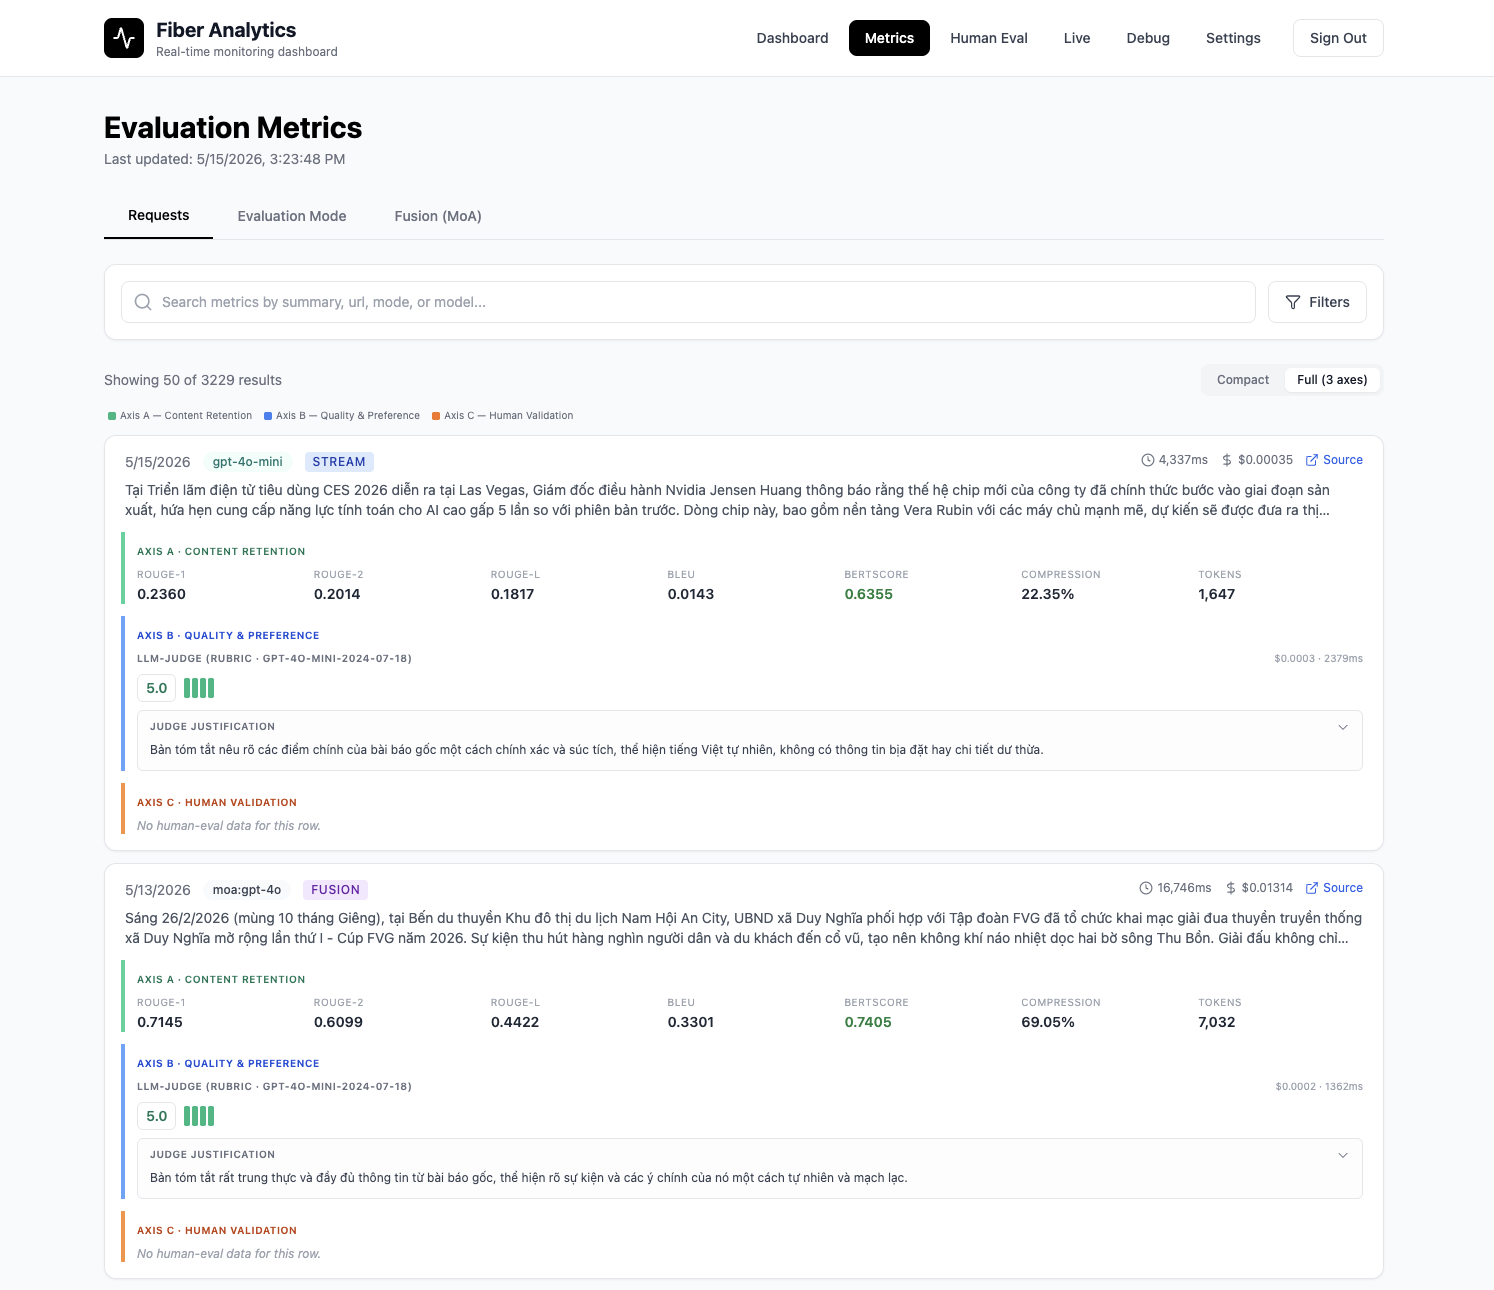
\includegraphics[width=0.85\linewidth]{figures/metrics_dashboard.png}
  \caption{Trang tổng quan số liệu đo lường với biểu đồ radar năm trục và các xu hướng chất lượng.}
  \label{fig:metrics_dashboard}
\end{figure}

\subsection{Giao diện đánh giá của con người}

Giao diện khảo sát người đánh giá con người (Hình~\ref{fig:human_eval}) phục vụ song song cả nhà nghiên cứu lẫn những người tham gia đánh giá. 
Thẻ quản trị (admin tab) cho phép nhà nghiên cứu lựa chọn bài báo gốc và các bản tóm tắt ứng viên tương ứng để thiết lập các tác vụ xếp hạng mù ẩn danh $K$ chiều. 
Trong khi đó, giao diện dành cho người đánh giá trình bày các ứng viên này dưới dạng các thẻ kéo thả trực quan được gán nhãn trung lập \textit{Bản A, Bản B, Bản C} phục vụ việc xếp hạng ẩn danh. 
Kết quả thu được sau đó sẽ được hệ thống tự động tổng hợp thành thứ hạng trung bình, tỷ lệ thắng tương ứng kèm theo các kiểm định ý nghĩa thống kê chính xác.

\begin{figure}[H]
  \centering
  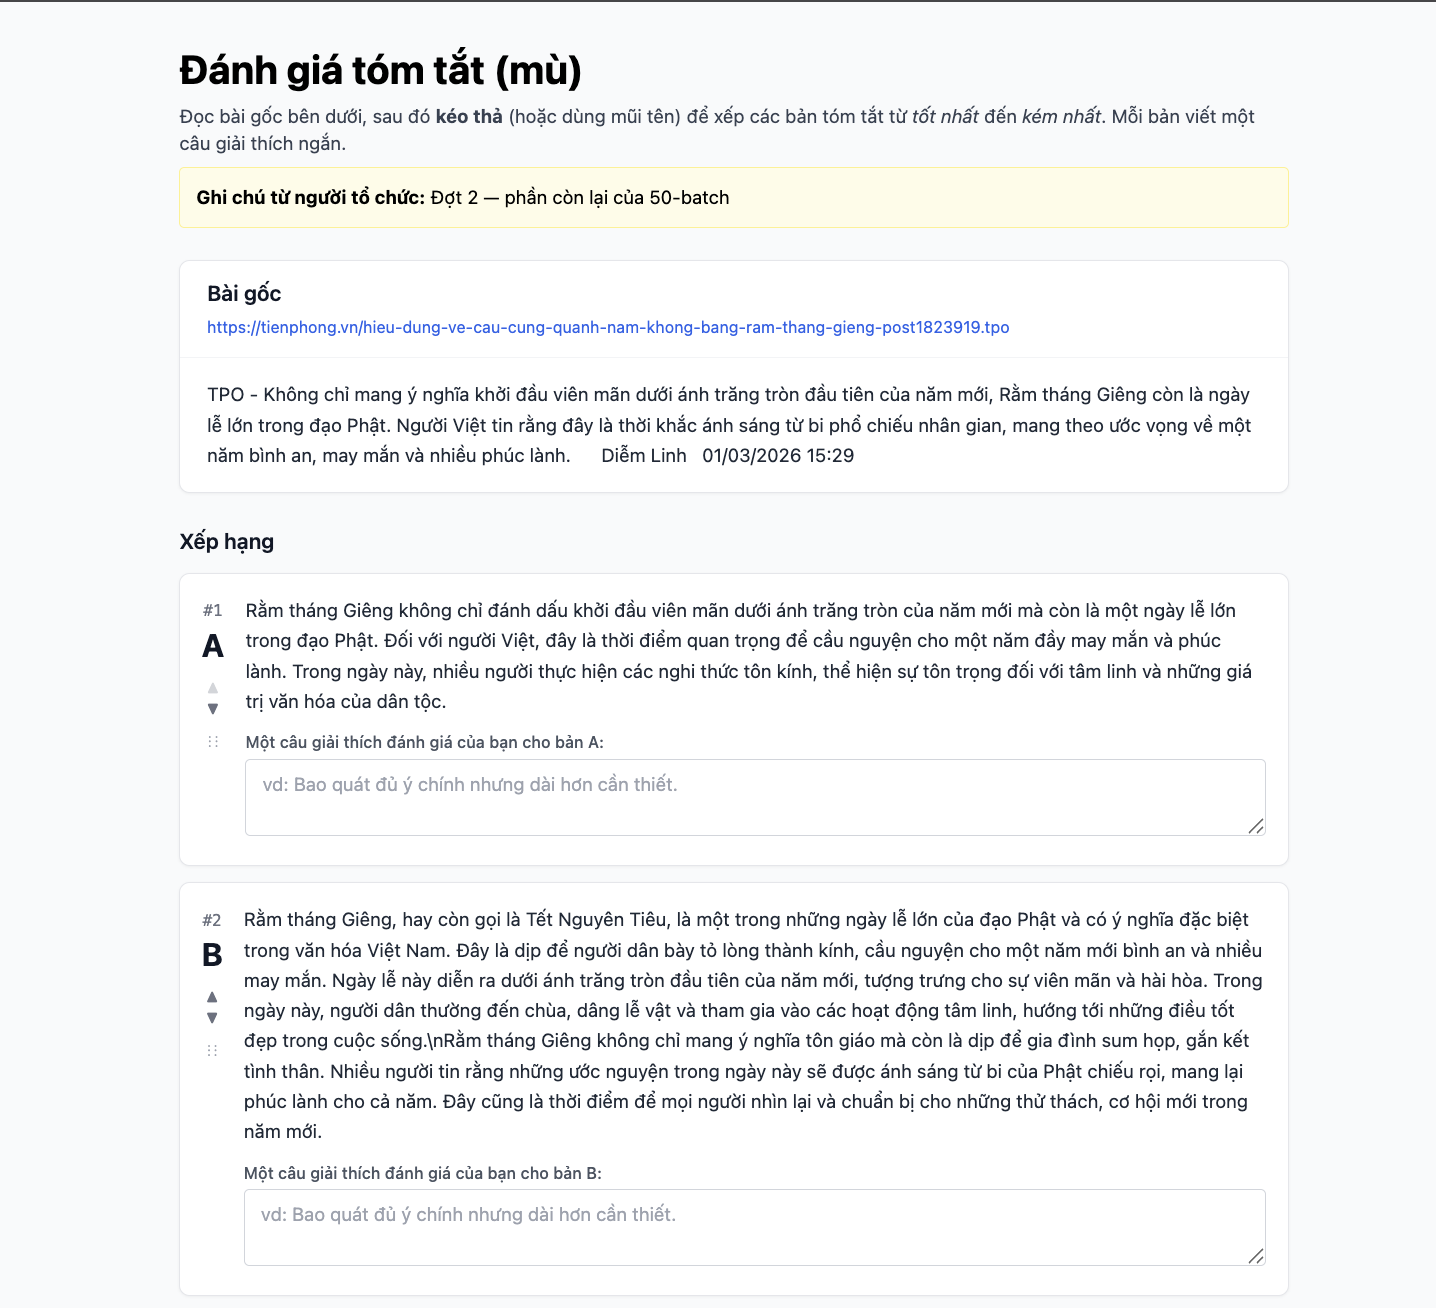
\includegraphics[width=0.85\linewidth]{figures/human_eval.png}
  \caption{Giao diện khảo sát đánh giá của con người phục vụ xếp hạng mù Bản A/B/C.}
  \label{fig:human_eval}
\end{figure}

\subsection{Trang thiết lập cấu hình (\texttt{/settings})}

Trang cài đặt cấu hình hệ thống (Hình~\ref{fig:settings}) cung cấp ba thẻ tùy chỉnh chuyên biệt:

\begin{itemize}
  \item \textbf{Định tuyến (Routing):} Tùy chọn thay đổi chế độ định tuyến (\texttt{auto} / \texttt{forced} / \texttt{fusion}) và trình chọn mô hình bắt buộc tương ứng.
  \item \textbf{Giám khảo LLM (Judge):} Thiết lập chế độ chạy (\url{metrics_only} - chỉ tính toán Trục A, \url{judge_only} - chỉ gọi giám khảo LLM Trục B, hoặc \texttt{both} - chạy cả hai), chọn mô hình giám khảo mặc định, phong cách chấm điểm (Rubric hoặc điểm tổng hợp Absolute), và nút chuyển đổi bật tắt chế độ kiểm chứng xác thực.
  \item \textbf{Khóa nhà cung cấp (Provider keys):} Hiển thị danh sách trạng thái cấu hình của các khóa API từ các nhà cung cấp dịch vụ LLM khác nhau ở chế độ chỉ đọc (read-only); toàn bộ nội dung của các khóa này được bảo mật an toàn phía máy chủ và không bao giờ được gửi về phía trình duyệt máy khách.
\end{itemize}

\begin{figure}[H]
  \centering
  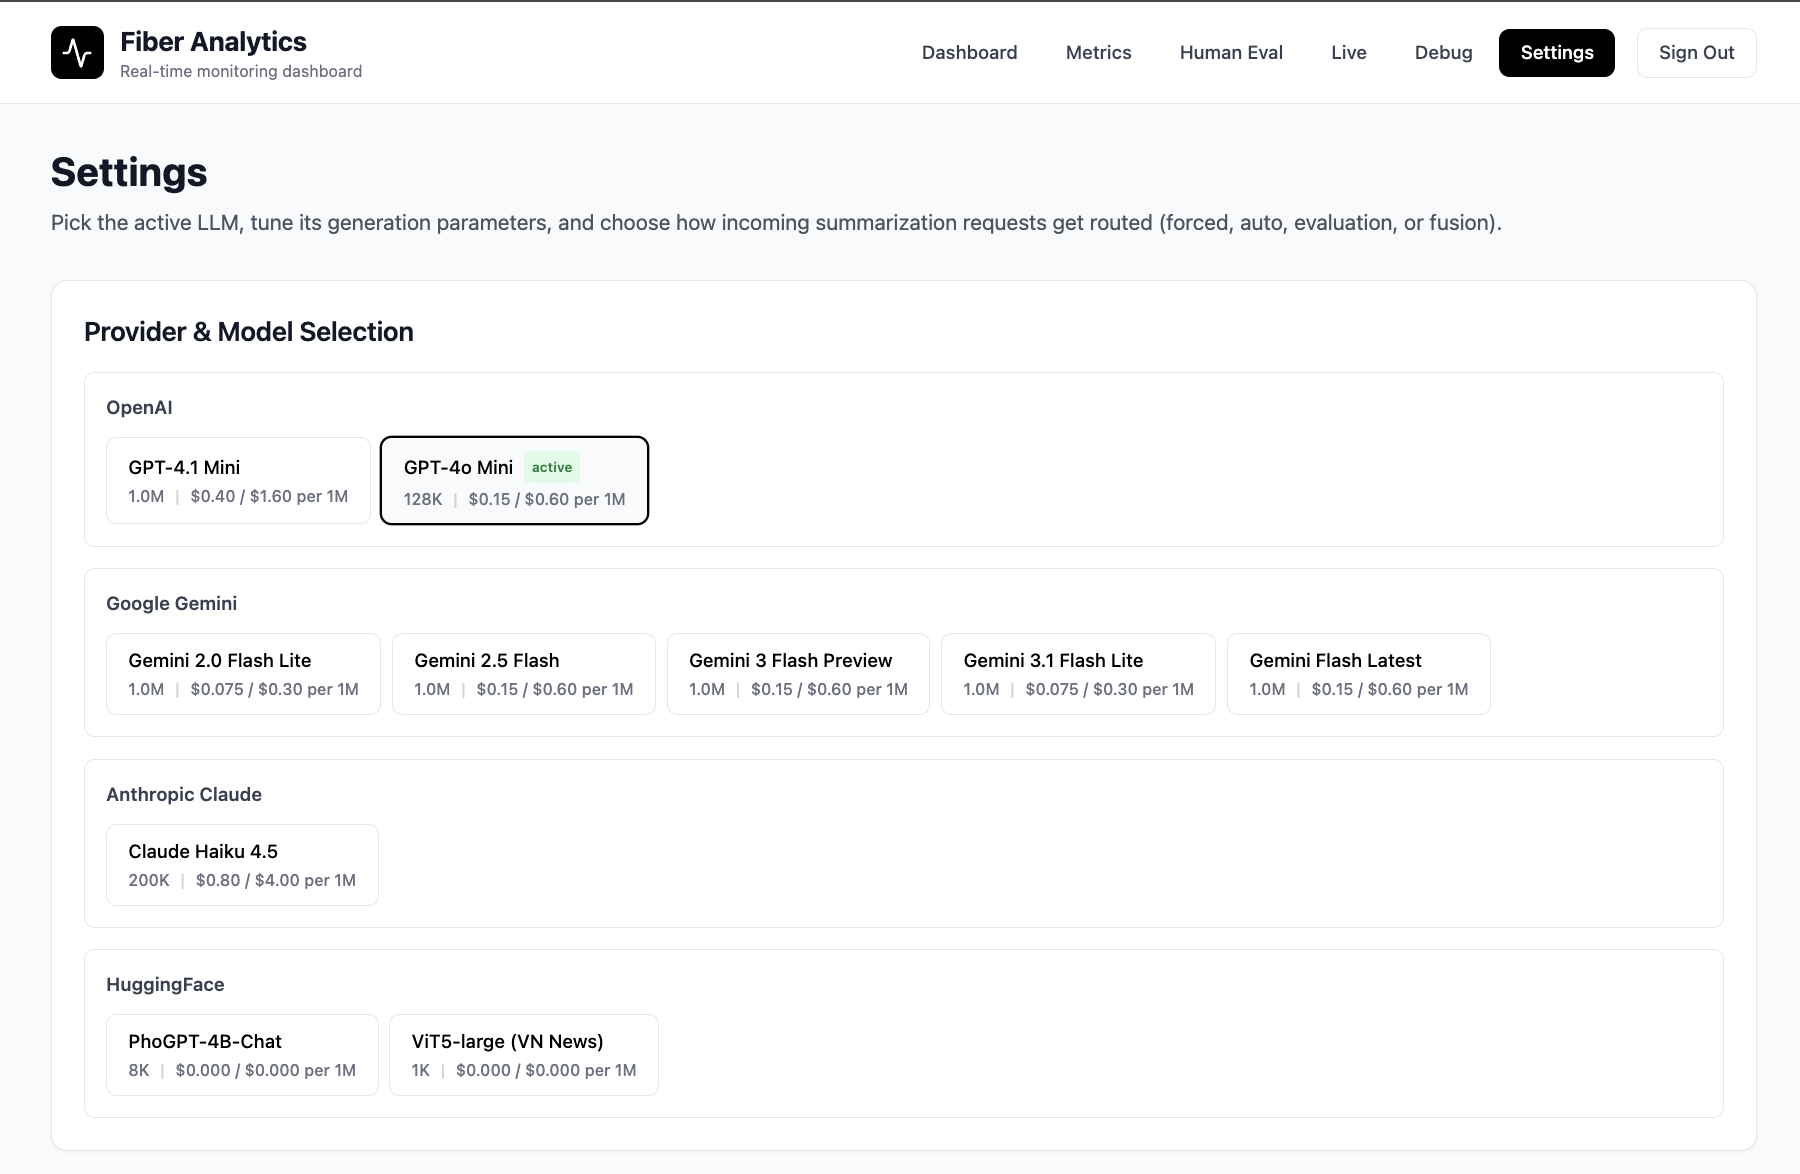
\includegraphics[width=0.85\linewidth]{figures/settings_page.png}
  \caption{Giao diện thiết lập các tùy chọn hệ thống và cấu hình khóa nhà cung cấp.}
  \label{fig:settings}
\end{figure}

\section{Tóm tắt chương}

Chương này đã trình bày toàn diện về thiết kế kiến trúc và giải pháp triển khai thực tế của hệ thống Fiber xoay quanh ba trụ cột cốt lõi: 
hệ thống sản phẩm thực tế hoạt động ổn định (gồm tiện ích mở rộng trình duyệt kết hợp backend Next.js và microservice tính toán BERTScore), 
pipeline dung hợp kết quả đa tác nhân MoA (đóng góp quan trọng về mặt kỹ thuật), và khung đánh giá chất lượng ba trục độc lập (đóng góp quan trọng về mặt phương pháp luận). 
Cấu trúc pipeline MoA tuân thủ nghiêm ngặt mô hình thiết kế của nghiên cứu gốc \cite{Wang2024} kết hợp với sự thích ứng miền bắt buộc là bổ sung kết nối phần dư bài viết gốc để đảm bảo thông tin tóm tắt luôn chính xác và trung thực. 
Đồng thời, sự tích hợp hài hòa của khung đánh giá ba trục giúp nhà nghiên cứu đo lường chất lượng hệ thống thông qua ba lăng kính độc lập và chuyên biệt, 
đảm bảo rằng bất kỳ kết luận khoa học nào được cả ba trục cùng đồng thuận ủng hộ đều đạt độ tin cậy thực chứng tối đa và không bị ảnh hưởng bởi thiên kiến của bất kỳ một công cụ đo lường đơn lẻ nào.
